% 16 pages in LNCS format including references. Appendices separate. 
\documentclass[a4paper]{llncs}


\linespread{0.95}
\usepackage{alltt}
\usepackage{import}
\usepackage{times}
\usepackage{multirow}
\usepackage{microtype}
\usepackage{array}
\usepackage{graphicx,wrapfig}
\usepackage[noadjust]{cite}
\usepackage{tikz}
\usetikzlibrary{plotmarks}
\usepackage{pgfplotstable}
\usepackage{filecontents}
\usepackage{pgfplots}
\usepackage{amsfonts}
\usepackage{amssymb}
\usepackage{amsmath}
\usepackage{stmaryrd}
\usepackage{color}
\usepackage{listings}
\usepackage{verbatim}
\usepackage{psfrag}
\usepackage{epsfig}
\usepackage{wasysym} 
%\usepackage{subfigure}
\usepackage{paralist}
%\usepackage{dingbat}
\usepackage[algo2e,linesnumbered,ruled,lined]{algorithm2e}
\usepackage{hyperref}
%\usepackage[active,tightpage]{preview}
%\PreviewEnvironment{tikzpicture}
\usepackage[subnum]{cases}
\makeatother

\newcommand{\extendedonly}[1]{}
\newcommand{\paperonly}[1]{#1}
\newtheorem{exmp}{Example}

\newcommand{\tool}[1]{\textsc{#1}\xspace}
\newcommand{\cbmcv}{\tool{cbmc 5.0}}
\newcommand{\Omit}[1]{}
\newcommand{\mydef}[1]{\begin{definition}#1\end{definition}}
\newcommand{\rmcmt}[1]{{\color{magenta}{#1}}}%#1
\newcommand{\pscmt}[1]{{\color{blue}{#1}}}%#1
\newcommand{\dkcmt}[1]{{\color{red!70!black}{#1}}}%#1
\newcommand{\tmcmt}[1]{{\color{orange}{#1}}}%#1
\newcommand{\lhcmt}[1]{{\color{purple}{#1}}}%#1

\input{symbols}

\begin{document}

\title{Lifting CDCL to Template-based Abstract Domains\\ for Program Verification}

\author{Rajdeep Mukherjee\inst{1} \and Peter Schrammel\inst{2} \and 
Leopold Haller\inst{3} \and \\ 
Daniel Kroening\inst{1} \and Tom Melham\inst{1}}

\institute{University of Oxford, UK \and University of Sussex, UK \and Google Inc., USA}

\maketitle

%===============================================================================
\begin{abstract}
%===============================================================================
%
The success of Conflict Driven Clause Learning (CDCL) for Boolean
satisfiability has inspired its adoption in other domains.  We present a
novel lifting of the CDCL to program analysis called \emph{Abstract Conflict
Driven Learning for Programs} (ACDLP).  ACDLP alternates between \emph{model
search}, which performs over-approximate deduction with constraint
propagation, and \emph{conflict analysis}, which performs under-approximate
abduction with heuristic choice.  We instantiate the model search and
conflict analysis algorithms to an abstract domain of \textit{template
polyhedra}, strictly generalising CDCL from the Boolean lattice to richer
lattice structures.  Our domain of template polyhedra can express intervals,
octagons, and certain restricted polyhedral constraints over program
variables.  We have implemented ACDLP for automatic bounded safety verification 
of C programs.  We~evaluate the performance of our
analyser by comparing with the CBMC program verifier, which uses
propositional solvers, and Astr{\'e}e, a commercial abstract
interpretation tool.  We observe one order of magnitude reduction in the
number of decisions, propagations, and conflicts as well as~1.5X speedup 
in runtimes for ACDLP compared to CBMC.  Compared to Astr{\'e}e, ACDLP is {63}\% 
more precise.  To the best of our knowledge, this is the first instantiation 
of CDCL with a template polyhedra abstract domain for safety verification.
%
\end{abstract}

%===============================================================================
\section{Introduction}

%%%%%%%%%%%%%%%%%%%%%%% AI %%%%%%%%%%%%%%%%%%%%%%%%
%
Static program analysis with abstract interpretation~\cite{CC77} is widely
used to verify properties of safety-critical systems.  Static analyses
commonly aim to compute program invariants as fixed-points of abstract
transformers.  Abstract states are chosen from a lattice that has meet
$(\sqcap)$ and join $(\sqcup)$ operations; the meet precisely models set
intersection (or conjunction, taking a logical view), and the join
over-approximates set union (or disjunction).  Over-approximation in the
join operation is one of the sources of precision loss, which causes false
alarms.  Typical abstract domains are non-distributive; suppose $a$ and $b$
together represent the abstract semantics of a program and $c$ represents a
set of abstract behaviours that violate the specification.  In a
non-distributive domain, $(a \sqcup b) \sqcap c$ can be strictly less
precise than $(a \sqcap c) \sqcup (b \sqcap c)$.  This means that in typical
abstract domains, analysing program behaviours separately can improve the
precision of the analysis.  Usual means to address false alarms therefore
include not only the use of richer abstract domains, but also of refinements
that delay joins or perform some form of case-splitting.  Such techniques
trade off higher precision against lower efficiency and may be susceptible
to case enumeration behaviour.

%%%%%%%%%%%%%%%%%%%%%%% CDCL %%%%%%%%%%%%%%%%%%%%%
By contrast, Model Checking (MC)~\cite{mc-book} can be seen to operate on
distributive lattice structures that represent disjunction without loss
of precision.  Classical MC directly operates on distributive
representations, such as BDDs, while more recent implementations use SAT
solvers.  SAT solvers themselves operate on partial assignments, which are
non-distributive structures.  To handle disjunction, case-splitting is
performed~\cite{sas12}.  Propositional SAT solvers solve large formulae, and
are often able to avoid enumerating cases.  The impressive performance of
modern solvers is credited to well-tuned decision heuristics and
sophisticated clause learning algorithms.  Collectively, these algorithms
are referred to as \emph{Conflict Driven Clause Learning}
(CDCL)~\cite{cdcl}.  An obvious idea is to lift CDCL from the domain of 
partial assignments to other non-distributive domains.

%%%%%%%%%%%%%%%%%%%%%%% ACDCL %%%%%%%%%%%%%%%%%%%%%
Abstract Conflict Driven Clause Learning (ACDCL)~\cite{dhk2013-popl} is one
such lattice-based generalization of CDCL.  ACDCL is a general algorithmic
framework, parameterized by a concrete domain~$C$ and an abstract
domain~$A$.  Classical CDCL can be viewed as an instance of ACDCL in which
$C$ is the set of propositional truth assignments and $A$ the domain of
propositional partial assignments~\cite{leo-thesis}.  Since the concrete
domain of interest is a parameter to the framework, ACDCL can in principle
be used to build both \emph{logical decision
procedures}~\cite{DBLP:journals/fmsd/BrainDGHK14} and \emph{program
analyzers}.  In the former case, the concrete domain is the set of candidate
models for the formula; in the latter case, it is the set of program traces
that may lead to an error.  Haller
et~al.~in~\cite{DBLP:journals/fmsd/BrainDGHK14} illustrate the first idea by
presenting a floating-point decision procedure that uses interval constraint
propagation.

%%%%%%%%%%%%%%%%%%%%%%% ACDLP %%%%%%%%%%%%%%%%%%%%%

In this paper, we explore the second idea by presenting an extension of 
ACDCL to program analysis.  We call our 
framework \emph{Abstract Conflict Driven Learning for Programs}
(ACDLP).  The key insight of ACDLP is to use decisions and learning to precisely 
reason about disjunctions in non-distributive domains, thereby automatically 
refining the precision of analysis for safety checking of C programs.  
We~introduce two central components of our framework: an abstract
model search algorithm that uses decisions and propagations to 
search for counterexample trace and an abstract conflict analysis 
procedure that approximates a set of unsafe traces through transformer 
learning.
%%%%%%%%%%%%%%%%%%%%%%% Domain %%%%%%%%%%%%%%%%%%%%%
We illustrate the application of our framework to program analysis 
using a \textit{template polyhedra abstract domain}~\cite{vmcai05}, 
which includes most of the commonly used abstract domains, such as boxes, 
octagons, zones and TCMs.  

We present an experimental evaluation of our analyser compared 
to CBMC~\cite{cbmc.tacas:2004}, which uses propositional solvers, and to 
Astr{\'e}e~\cite{DBLP:conf/pldi/BlanchetCCFMMMR03}, a commercial abstract 
interpretation tool.  In this paper, we make the following contributions.

\Omit{
Our experiments suggest that ACDLP can be seen as a 
technique to improve efficiency of SAT-based BMC. Additionally, it can 
also be perceived as an automatic way to improve the precision of abstract 
interpretation for bounded unwindings of programs.  
}
%
\begin{enumerate}
\item A novel program analysis framework that lifts model search and conflict
analysis procedures of CDCL algorithm over a template polyhedra abstract domain. These techniques
are embodied in our tool, \emph{ACDLP}, for automatic bounded safety verification 
    of C programs.
\item A parameterized abstract transformer that guides the model
  search in forward, backward and multi-way direction for counterexample
    detection. 
\item A conflict analysis procedure that performs UIP-based transformer learning 
  over template polyhedra abstract domain through abductive reasoning. 
\end{enumerate}
%

\Omit{
While the focus of this paper is the analysis of loop-free unwindings of programs, our technique is in 
principle compatible with abstract-interpretation-based handling of loops using 
widenings~\cite{leo-thesis}.  Although, finding non-trivial trace abstraction 
that satisfy properties of ACDCL is an open problem.  Finally, we present the 
results of experimental evaluation of our analyser compared to CBMC~\cite{cbmc.tacas:2004}, 
which uses propositional solvers, and to Astr{\'e}e~\cite{DBLP:conf/pldi/BlanchetCCFMMMR03}, 
a commercial abstract interpretation tool. 
}
%%%%%%%%%%%%%%%%%%%%%%% Experiments %%%%%%%%%%%%%%%%%%%%%
%\vspace{-7mm}

% This abstract domain captures many
% relationships between program variables that intervals cannot represent.
% TM - INTERVALS don't express relationships at all. 

%Fundamentally, the abstract domain of polyhedra~\cite{polyhedra} is a 
%complete relational domain that capture all linear inequalities 
%between program variables.  
%It is a `relational' domain, in the sense that
%its elements express relationships between two or more program variables. 
%By contrast, the interval domain expresses constraints on individual program variables.


\Omit {


%This enables an ACDCL-based analyser to automatically refine an imprecise 
%analysis and thus prevents enumeration behaviour.  

%To date, ACDCL has been instantiated as a decision procedure for the
%first-order theory of floating-point arithmetic~\cite{DBLP:journals/fmsd/BrainDGHK14}, 

%\rmcmt{state other limitations}.  
that is, given abstract domain elements $a$, $b$, $c$, 
$(a \sqcup b) \sqcap c \sqsupseteq (a \sqcap c) \sqcup (b \sqcap c)$.

We provide a theoretical recipe and a practical instantiation for 
generalising CDCL architecture to arbitrary abstract domains.   

\paragraph{Abstract Domain.} 
Limited expressivity of abstract domains may lead to imprecise 
over-approximation which gives rise to false alarms. Evidently, the 
verification of many programs requires more expressive numerical domains, 
such as polyhedra for analysis.  These domains capture numerical 
relationship between program variables that intervals cannot express.  
To this end, we provide a theoretical recipe and a practical instantiation 
for generalising CDCL architecture to arbitrary abstract domains, thus 
lifting it to richer lattice structures. 

The key motivation of our work is to combine the precision of a SAT solver 
and the efficiency of an abstract interpreter to present a new class of 
program analysers.  

\rmcmt{Introduce ACDLP here with a distinct notion for programs}
Whereas the propositional reasoning of SAT solvers can be lifted easily from the 
Boolean lattice to other non-relational domains, application to relational 
domains is challenging because of the relational properties of inferred 
deductions and the complexity of the closure operation in fixed-point computation 
during the propagation phase.  In this paper, we identify specific modifications 
to the CDCL algorithm that are necessary to lift propositional CDCL to 
template polyhedra domain. 

\rmcmt{Present program and property driven trace partitioning (with inline example with octagons)} 
}

%===============================================================================

%===============================================================================
%\paragraph{Contributions}
In this paper, we make the following technical contributions.
%
\begin{compactenum}
\item We present a novel program analysis technique called {\em Abstract 
Conflict Driven Learning for Programs} (ACDLP) that lifts the CDCL algorithm 
over template polyhedra abstract domains for safety verification of C programs.  
%We have implemented our analyzer ACDLP for safety verification of C programs. 
We compare the performance of ACDLP compared to a precise model checker CBMC and a 
commercial abstract interpreter Ast{\'r}ee.  Our tool is available 
online\footnote{http://www.cprover.org/acdcl/}. 

\Omit{  
We present a generic implementation framework for model search, conflict analysis, 
learning and backjumping phase that can be instantiated over any arbitrary 
abstract domains, thus making our tool easily extendable to domain specific decision, 
propagation and learning heuristics.  
}
\item We present an abstract model search algorithm that strictly 
generalises the Boolean Constraint Propagation (BCP) procedure. We 
propose several domain specific propagation and decision heuristics 
that infers abstract domain elements over the template polyhedra domain.   
\Omit{
We propose a domain-specific decision heuristics that exploit the 
expressivity of the underlying abstract domain to make effective decisions. 
}
\item We sketch an abstract conflict analysis procedure that operates on an 
abstract conflict graph to learn a generalised reason for conflicts.  
 
\item  Experiments indicate a two order of magnitude reduction 
in the number of decisions, propagations, and conflicts compared 
to a SAT solver while being more precise than an abstract interpreter.  
\Omit {
set of benchmarks drawn from the bitvector regression category in 
SV-COMP, bit-precise software models auto-generated from hardware 
circuits domain and some hand crafted example show that 
}
\end{compactenum}

%===============================================================================

%===============================================================================
\section{Motivating Examples}

In this section, we present two simple examples to demonstrate the core idea
of ACDLP for bounded program verification.  For each example, we apply three
analysis techniques: \textit{abstract interpretation} (AI), SAT-based
\textit{bounded model checking} (BMC) and ACDLP. \\ 
%
\textbf{First Example}
The simple Control-Flow Graph (CFG) in Fig.~\ref{fig:example1} squares
a machine integer and checks that the result is positive.  To avoid
overflow, we assume the input~v has an upper bound~N.  This example 
demonstrates that a) interval analysis in ACDLP is more precise than a 
forward AI in the interval domain, and b) ACDLP with intervals 
can achieve a precision similar to that of octagonal AI without 
employing more sophisticated mechanisms such as trace partitioning~\cite{toplas07}.
%
\begin{figure}[t]
\centering
\begin{tabular}{c|c|c}
\hline
Control-Flow Graph & Interval Analysis in ACDLP & Octagon Analysis in ACDLP\\
\hline
\scriptsize
\begin{minipage}{3.3cm}
%\centering
%\vspace*{0.3cm}
\scalebox{.52}{\import{figures/}{example.pspdftex}}
%\caption{\label{fig:cfg}}
\end{minipage}
&
\begin{minipage}{5.7cm}
%\centering
\vspace*{0.3cm}
\scalebox{.5}{\import{figures/}{acdl_run.pspdftex}}\vspace*{0.1cm}
%\caption{\label{fig:itv}}
\end{minipage}
&
\begin{minipage}{3.6cm}
%\centering
\vspace*{0.3cm}
\scalebox{.5}{\import{figures/}{acdl_oct.pspdftex}}
%\caption{\label{fig:oct}}
\end{minipage}
\\
\hline
\end{tabular}
\caption{\label{fig:example1}
CFG and corresponding Abstract Conflict Graphs for Interval and Octagon Analysis}
\end{figure}
%


\noindent \textbf{AI versus ACDLP}
Conventional forward interval AI is too imprecise to verify safety of this program
owing to the control-flow join at node~n4.  For example, the
state-of-the-art AI tool Astr{\'e}e requires external hints, provided
by manually annotating the code with partition directives at n1.  This 
informs Astr{\'e}e to analyse program paths separately.

%\textbf{General Working Mechanism of ACDLP}
However, ACDLP can be understood as an algorithm to automatically infer such
partitions.  For the example in Fig.~\ref{fig:example1}, interval analysis
with ACDLP is sufficient to prove safety.  The analysis records the
decisions and deductions in a \textit{trail} data-structure.  The trail can
be viewed to represent a graph structure called the {\em Abstract Conflict
Graph} (ACG) that stores dependencies between decisions and deductions
nodes, similar to the way an \emph{Implication Graph}~\cite{cdcl} works in a SAT solver. 
Nodes of the ACG in the second column of Fig.~\ref{fig:example1} are
labelled with the CFG location and the corresponding abstract value. 
Beginning with the assumption that v=[0,5] at node~n1, the intervals
generated by forward analysis in the initial deduction phase at
\emph{decision level}~0 (DL0) are $x=[-5,5]$ and $z=[-25,25]$.  Clearly
these do not prove safety, as shown in ACG1.  ACDLP therefore makes a
heuristic decision, at DL1, to refine the analysis.  With the decision
$c=[1,1]$, interval analysis then concludes $x=[0,5]$ at node n4, which
leads to $(\mathrm{Error}{:}\;\bot)$ in ACG2, indicating that the error
location is unreachable and that the program is safe when $c=[1,1]$.

Reaching $(\mathrm{Error}{:}\;\bot)$ is analogous to reaching a conflict in
a propositional SAT solver.  At this point, a clause-learning SAT solver
learns a reason for the conflict and backtracks to a level such that the
learnt clause is \textit{unit}.  By a similar process, ACDLP learns that
$c=[0,0]$.  That is, all error traces must satisfy $(c \neq 1)$.  The
analysis discards all interval constraints that lead to the conflict and
backtracks to DL0.  ACDLP then performs interval analysis with the learnt
clause $(c \neq 1)$.  This also leads to a conflict, as shown in ACG3.  The
analysis cannot backtrack further and so terminates, proving the program
safe.  Thus, {\em decision} and {\em clause learning} are used to infer the
partitions necessary for a precise analysis.  Alternatively, the octagon
analysis in ACDLP---illustrated in the third column of
Fig.~\ref{fig:example1}---can prove safety with propagations only. 
No~decisions are required.  Forward AI with octagons in Astr{\'e}e is also
able to prove safety.  
%
\begin{table}[!b]
%\scriptsize
\begin{center}
{
\begin{tabular}{l|r|r|r|r|r|r}
\hline
  Solver & Domains & decisions & propagations & conflicts & conflict literals & restarts \\ \hline
  \multicolumn{7}{c}{Solver statistics for Fig.~\ref{fig:example1} (For N = 46000)} \\ \hline
  MiniSAT & $\boolvars \rightarrow \{t,f,?\} $ & 233 & 36436 & 162 & 2604 & 2 \\ \hline
  ACDLP & $\mathit{nodes} \rightarrow \intervals[\numvars]$ & 1 & 17 & 1 & 1 & 0 \\ \hline
  ACDLP & $\mathit{nodes} \rightarrow \octagons[\numvars]$ & 0 & 7 & 0 & 0 & 0 \\ \hline 
  \multicolumn{7}{c}{Solver statistics for Fig.~\ref{fig:example2}} \\ \hline
  MiniSAT & $\boolvars \rightarrow \{t,f,?\} $ & 4844 & 32414 & 570 & 4750 & 5 \\ \hline
  ACDLP & $\mathit{nodes} \rightarrow \octagons[\numvars]$ & 4 & 412 & 2 & 2 & 0 \\ 
\hline
\end{tabular}
}
\end{center}
\caption{SAT-based BMC versus ACDLP for verification of programs in Fig.~\ref{fig:example1} and
  Fig.~\ref{fig:example2}}
\label{solver}
\end{table}
%
%
\begin{figure}[t]
\centering
\begin{tabular}{c|c}
\hline
Control-Flow Graph & Octagon Analysis in ACDLP \\
\hline
\scriptsize
\begin{minipage}{5.28cm}
%\centering
%\vspace*{0.3cm}
\scalebox{.52}{\import{figures/}{cfg.pspdftex}}
%\caption{\label{fig:cfg}}
\end{minipage}
&
\begin{minipage}{7.5cm}
%\centering
\vspace*{0.3cm}
\scalebox{.5}{\import{figures/}{oct_partition.pspdftex}}\vspace*{0.1cm}
%\caption{\label{fig:itv}}
\end{minipage}
\\
\hline
\end{tabular}\caption{\label{fig:example2}
CFG and corresponding Abstract Conflict Graphs for Octagon Analysis}
\end{figure}
%


\noindent \textbf{Second Example} Fig.~\ref{fig:example2}, demonstrates that 
octagon analysis in ACDLP is more precise than forward AI in the octagon domain.
% LATER, b) \emph{ACDLP with octagons can outperform SAT-based BMC}.  
The CFG in Fig.~\ref{fig:example2} computes the absolute 
values of two variables, $x$ and~$y$, under the assumption 
$(x=y) \lor (x=-y)$. 

\noindent \textbf{AI versus ACDLP}
Forward AI in the octagon domain infers 
the octagonal constraint $\mathrm{Error}{:}\;(p\geq0 \wedge p+q\geq0 \wedge q\geq0 \wedge p+x\geq0 \wedge 
p-x\geq0 \wedge q+y\geq0 \wedge q-y\geq0)$. Clearly this is too 
imprecise to prove safety. 
%
The octagonal analysis in ACDLP is illustrated by the ACGs in
Fig.~\ref{fig:example2}.  Due to space limitations, we elide intermediate
deductions with dotted lines.  The decision $x=y$ at DL1 is not sufficient
to prove safety, as shown in ACG1.  Hence, a new decision $x<0$ is made at
DL2, followed by forward propagation that infers $y<0$ at node n5.  This
subsequently leads to safety ($\mathrm{Error}{:}\;\bot$), as shown in ACG2. 
The analysis learns the reason for the conflict, discards all deductions in
ACG2 and backtracks to DL1.  Octagon analysis is run with the learnt
constraint $(x\geq0)$ and this infers $y\geq0$ at node n5, as shown in ACG3. 
This also leads to safety ($\mathrm{Error}{:}\;\bot$).  The analysis now
makes a new decision $x=-y$ at DL1.  The procedure is repeated leading to
results shown in ACG4, ACG5, and ACG6.  Clearly, the decisions $x=-y$ and
$x<0$ also lead to safety.  The analysis backtracks to DL0 and returns {\em
safe}.  Note that the specific decision heuristic we use in this case
exploits the control structure of the program to infer partitions that are
sufficient to prove safety. \\ \\
%
\noindent \textbf{ACDLP versus BMC}
ACDLP can require many fewer iterations than SAT-based BMC due to its
ability to reason over much richer lattice structures.
%in terms of number of {\em decisions}, {\em propagations}, and {\em conflicts}. 
A SAT-based BMC converts the program into a bit-vector equation 
and passes that to a CDCL-based SAT solver for proving safety.  
Table~\ref{solver} compares the statistics for BMC with 
MiniSAT~\cite{minisat} solver to those for interval and octagon 
analysis in ACDLP. In the column labelled $\textrm{Domains}$, 
$\boolvars$ is the set of propositional variables; each of these is mapped to
{\em true} (t), {\em false} (f) or {\em unknown} $(?)$. $\numvars$ is the set of
numerical variables, $\mathit{nodes}$ the set of nodes in the CFG;
$\intervals[\numvars]$ and $\octagons[\numvars]$ are the Interval and Octagon
domains over $\numvars$. As can be seen, ACDLP outperforms BMC in the total number of 
{\em decisions}, {\em propagations}, {\em learnt clauses} and {\em restarts} 
for both example programs.

\Omit{
However, in contrast to a SAT solver, the octagonal analysis in ACDLP is 
very efficient, as shown in Table~\ref{solver2}.  \rmcmt{This shows the advantage 
of using richer abstract domains within the CDCL-style analysis}.  
%
\begin{table}[!b]
\begin{center}
{
\begin{tabular}{l|r|r|r|r|r|r}
\hline
  Solver & Domain & decisions & propagations & conflicts & conflict literals & restarts \\ \hline
  MiniSAT & $\boolvars \rightarrow \{t,f,?\} $ & 4844 & 32414 & 570 & 4750 & 5 \\ \hline
  ACDLP & $\mathit{nodes} \rightarrow $ & 4 & 412 & 2 & 2 & 0 \\ 
\hline
\end{tabular}
}
\end{center}
\caption{Solver statistics for Example given in Fig.~\ref{fig:example2}}
\label{solver2}
\end{table}
}

%===============================================================================

%===============================================================================
\section{Program Model and Abstract Domain}\label{sec:domains}
%-------------------------------------------------------------------------------
\subsection{Program Representation}\label{sec:program}  
%
We consider \emph{bounded programs} with safety
properties given as a set of assertions, $\assertions$, in the program.
%
A bounded program is obtained by a transformation that unfolds
loops and recursions a finite number of times. The result 
is represented by a set
$\constraints=\program\cup\{\neg \bigwedge_{\assertion\in\assertions} \assertion\}$,
where $\program$ contains an encoding of the statements in the program as
constraints, obtained after translating the program
into single static assignment (SSA) form via a data flow analysis.
%
The representation $\constraints$ for the program in Fig.~\ref{fig:example1} is 
%
\begin{equation}\label{eq:ssa}
\begin{array}{l@{}l}
\{ & g_0 = (0 \leq v \leq N),\:
     g_1 = (g_0 \wedge c),\:
     x_0 = v,\:
     x_1 = -v, \\ 
  &  x_2 = g_1?x_0:x_1, \:
     g_2 = (g_1 \vee g_0\wedge \neg c), \:
     z  = x_2{\cdot}x_2,\:
     g_2 \wedge z{<}0 \}
\end{array}
\end{equation}
%
Assignments such as x:=v become equalities $x_1=v$, where the
left-hand side variable gets a subscripted fresh name.
%
Control flow is encoded using guard variables, e.g.~$g_1=g_0\wedge c$.
%
Data flow joins become conditional expressions, e.g.~$x_3=g_1?x_1:x_2$.
%
The assertions in $\assertions$ are constraints such as $g_2
\Rightarrow z\geq 0$, meaning that if $g_2$ holds
(i.e.,~the assertion is reachable) then the assertion must hold.
%
We~write $\vars$ for the set of variables occurring in $\constraints$.  
Based on the above program representation, we define a \textit{safety formula}
($\formula$) as the conjunction of everything in $\constraints$, that is,  
$\formula:= \bigwedge_{\constraint\in\constraints} \constraint$. The formula 
$\formula$ is unsatisfiable if and only if the program is safe.
%
\begin{table}[t]
\small
\begin{center}
{
\begin{tabular}{c@{\quad}|@{\quad}c@{\quad}|@{\quad}c@{\quad}|@{\quad}c@{\quad}|@{\quad}c}
Interval & Octagons & Zones & Equality & Fixed-coef.~Polyhedra \\ \hline
$a \leq x_i \leq b$ & $\pm x_i \pm x_j \leq d$ & $x_i - x_j \leq d$ & 
  $x_i=x_j\Omit{,(x_i \neq x_j)}$ & $a_1x_1 + \ldots + a_nx_n \leq d$
\end{tabular}
}
\end{center}
\caption{Template instances in the template polyhedra domain}
\label{domain}
\end{table}
%
%-------------------------------------------------------------------------------
\subsection{Abstract Domain}
%-------------------------------------------------------------------------------
%Silva et al.~\cite{sas12,dhk2013-popl} showed that SAT solvers operate on the domain 
%of partial assignments~\cite{sas12,dhk2013-popl}.  
In this paper, we instantiate ACDLP over a reduced product domain~\cite{CC79}
$\domain[\vars]=\booldomain^{|\boolvars|}\times\reldomain[\numvars]$ where
$\booldomain$ is the Boolean domain that permits abstract values
$\{\true,\false,\bot,\top\}$ over boolean variables $\boolvars$ in the
program, and $\reldomain$ is a \textit{template polyhedra}~\cite{vmcai05}
domain over the numerical (bitvector) variables $\numvars$.  Our template
polyhedra domain can express various relational and non-relational templates
over $\numvars$, as given in Table~\ref{domain}.
% 
%-------------------------------------------------------------------------------
\subsubsection{Template Polyhedra Abstract Domain}
%-------------------------------------------------------------------------------
%
An abstract value of the template polyhedra domain~\cite{vmcai05}
represents a set $\numconcval$ of values of the vector $\vec{\numvar}$ 
of numerical (bitvector) variables $\numvars$ of their respective
data types. (Currently, signed and unsigned integers are supported.)
For example, in the program given by Eq.~(\ref{eq:ssa}), we have four 
numerical variables, written as the vector $\vec{\numvar} = (x_0,x_1,x_2,z)$.  
An abstract value is a constant vector $\vec{\numabsval}$ that represents 
sets of values for $\vec{\numvar}$ for which 
$\mat{C}\vec{\numvar}\leq\vec{\numabsval}$, for a fixed coefficient 
matrix $\mat{C}$.  The domain containing $\vec{\numabsval}$ is augmented 
by a special element $\bot$ to denote the minimal element of the lattice.  
%
There are several optimisation-based 
techniques~\cite{vmcai05} for computing the domain operations, 
such as meet ($\meet$) and join ($\sqcup$), in the template polyhedra domain.  
In our implementation, we use the strategy iteration approach of~\cite{BJKS15}.
%
The abstraction function is defined by $\alpha(\numconcval) = \min \{\vec{\numabsval}\mid
\mat{C}\vec{\numvar}\leq\vec{\numabsval}, \vec{\numvar}\in \numconcval\}$, where 
$\min$ is applied component-wise.  The concretisation $\gamma(\vec{\numabsval})$ is the set $\{\vec{\numvar}\mid
\mat{C}\vec{\numvar}\leq\vec{\numabsval}\}$ and $\gamma(\bot)=\emptyset$,
i.e., the empty polyhedron.

For notational convenience we will use conjunctions of linear
inequalities, for example $x_1\geq 0 \wedge x_1-z\leq 30$, to write the
abstract domain value $\vec{\numabsval}=\vecv{0}{30}$,
with $\mat{C}=\qmat{-1}{0}{1}{-1}$ and $\vec{\numvar}=\vecv{x_1}{z}$; 
$\true$ corresponds to abstract value $\top$ and $\false$ to 
abstract value $\bot$.
%
For a program with $N=|\numvars|$ variables, the template 
matrix $\mat{C}$ for the interval domain $\intervals[\numvars]$, 
has $2N$ rows. Hence, it generates at most $2N$ inequalities, one
for the upper and lower bounds of each variable.
%
For octagons $\octagons[\numvars]$, we have at most $2N^2$
inequalities, one for the upper and lower bounds of each variable and
sums and differences for each pair of variables. 
Unlike a non-relational domain, a relational domain such as octagons 
requires the computation of a \emph{closure} in order to obtain a normal 
form, necessary for precise domain operation. 
The closure computes all implied domain constraints.  
An example of a closure computation for octagonal inequalities is
$\mathit{closure}((x-y \leq 4) \wedge (y-z \leq 5))=((x-y \leq 4) \wedge (y-z
\leq 5) \wedge (x-z \leq 9))$.
%
For octagons, closure is the most critical and expensive operator; it has  
cubic complexity in the number of program variables.  We therefore compute 
closure lazily in template polyhedra domain in our abstract model search 
procedure, which is described in section~\ref{lazyclosure}. 
%We refer the reader to Appendix~\ref{appendix:lazyclosure} 
%for details of lazy closure computation. 
%-------------------------------------------------------------------------------
\subsubsection{Abstract Transformers}
%
An abstract transformer $\abstrans{\domain}{\constraint}$ transforms an
abstract value $\absval$ through a constraint $\constraint$; it
\emph{deduces} information from $\absval$ and $\constraint$.  The best
transformer is
%
\begin{equation}\label{eq:abstrans}
\abstrans{\domain}{\constraint}(\absval)=\absval\meet\alpha(\{\val\mid \val\in\gamma(\absval), \val\models \constraint\})
\end{equation}
 where we write 
$\val\models \constraint$ if the concrete value $\val$ satisfies the constraint $\constraint$.
%
Any abstract transformer that over-approximates the best abstract
transformer is a sound transformer and can be used in our algorithm.
%
For example, we can deduce $\abstrans{\domain}{x=2(y+z)}(\absval)=(0\leq y
\leq 2 \wedge\allowbreak 1 \leq y-z \leq 1\wedge\allowbreak -2\leq x\leq 6)$
for the abstract value $\absval=(0\leq y \leq 2 \wedge\allowbreak 1 \leq y-z
\leq 1)$.
%
We~denote the set of abstract transformers for a safety formula
$\formula$ using the abstract domain $\domain$ by
$\abstransset=\{\abstrans{\domain}{\constraint}\mid
\constraint\in\constraints\}$.
%


%-------------------------------------------------------------------------------
\subsection{Properties of Abstract Domains}
%-------------------------------------------------------------------------------
%
An important property of a clause-learning SAT solver is that each
non-singleton element of the partial assignment domain can be 
decomposed into a set of \textit{precisely complementable} singleton
elements~\cite{dhk2013-popl}.  This property of domain elements
is necessary to learn elements that help to guide the model search away from the
conflicting region of the search space.  
%
Most numerical abstract domains, such as intervals and octagons lack
complements in general, i.e., not every element in the domain has a
precise complement.  However, these domain elements can be represented
as intersections of half-spaces, each of which admits a precise complement.
We formalise this in the sequel.
%
\begin{definition} 
A \emph{meet irreducible} $m$ in a complete lattice 
structure $A$ is an element with the following property.
\begin{equation}
\forall m_1, m_2 \in A: m_1 \meet m_2 = m \implies (m = m_1 \lor m = m_2), m \neq \top  
\end{equation}
\end{definition}
%
\rmcmt{The meet irreducibles in the Boolean domain $\booldomain$ 
for a variable $x$ are $x$ and $\neg x$. The meet 
irreducibles in the template polyhedra domain are all elements 
that concretise to half-spaces, i.e., they can be represented 
by a single inequality. For the interval domain, these are 
$x \leq d$ or $x \geq d$ for constants $d$. (Refer thesis definition)}
%
\begin{definition}
A \emph{meet decomposition} $\decomp(\absval)$ of an abstract
element $\absval \in \domain$ is a set of meet irreducibles $M \subseteq \domain$ such that 
$\absval=\bigsqcap_{m\in M} m$.
\end{definition}

\noindent For polyhedra this intuitively means that each polyhedron can be
written as an intersection of half-spaces.
%
For example, the meet decomposition of the interval domain element
$decomp(2\leq x\leq 4 \wedge 3\leq y\leq 5)$ is
the set $\{x\geq 2, x\leq 4, y\geq 3, y\leq 5\}$.
%
\begin{definition} 
An element $\absval\in \domain$ is called \emph{precisely complementable}
iff there exists $\bar{\absval} \in \domain$ such that 
$\neg\gamma(\bar{\absval})=\gamma(\absval)$.
That is, there is an element whose complemented concretisation equals
the concretisation of $\absval$.
\end{definition}
%
The precise complementation property of a partial assignment lattice can
be generalised to other lattice structures. 
%
For example, the precise complement of a meet irreducible $(x \leq 2)$ in
the interval domain over integers is $(x \geq 3)$, or the precise complement
of the meet irreducible $(x+y \leq 1)$ in the octagon domain over integers
is $(x+y \geq 2)$.  Our domain implementation supports precise
complementation operation.  However, standard abstract interpretation does
not require a complementation operator.  Hence, abstract domain libraries,
such as APRON~\cite{apron}, do not provide it.  But it can be implemented
with the help of a meet decomposition as explained above.
%

%===============================================================================

%===============================================================================
\section{Abstract Conflict Driven Learning for Programs}

\begin{figure}[htbp]
\centering
\scalebox{.6}{\import{figures/}{acdlp-top.pspdftex}}
\caption{Architectural View of ACDLP\label{acdlp-top}}
\end{figure}

\begin{algorithm2e}[t]
\DontPrintSemicolon
\SetKw{return}{return}
\SetKwRepeat{Do}{do}{while}
%\SetKwFunction{assume}{assume}
%\SetKwFunction{isf}{isFeasible}
\SetKwData{conflict}{conflict}
\SetKwData{safe}{safe}
\SetKwData{sat}{sat}
\SetKwData{unsafe}{unsafe}
\SetKwData{unknown}{unknown}
\SetKwData{true}{true}
\SetKwInOut{Input}{input}
\SetKwInOut{Output}{output}
\SetKwFor{Loop}{Loop}{}{}
\SetKw{KwNot}{not}
\begin{small}
\Input{A program in the form of a set of abstract transformers $\abstransset$.}
\Output{The status \safe or \unsafe. %and a counterexample if \unsafe.
}
$\trail \leftarrow \langle\rangle$, $\reasons \leftarrow []$ \;
$\mathit{result} \leftarrow \deduce_{\propheur}(\abstransset,\trail,\reasons)$ \;
\lIf{$\mathit{result}$ = \conflict} {
  \return \safe}
\While{$true$} 
{
\lIf{$\mathit{result}$ = \sat} {
  \return \unsafe}
  $\decisionvar \leftarrow \decide_{\decheur}(\abs(\trail))$ \;
  $\trail \leftarrow \trail \cdot \decisionvar$ \; 
  $\reasons[|\trail|] \leftarrow \top$ \;
  $\mathit{result} \leftarrow \deduce_{\propheur}(\abstransset,\trail,\reasons)$\;
  \Do{$\mathit{result} = \conflict$} {
    \lIf{$\neg \analyzeconflict_{\confheur}(\abstransset,\trail,\reasons)$} {
      \return \safe
    }
    $\mathit{result} \leftarrow \deduce_{\propheur}(\abstransset,\trail,\reasons)$ \;
  }
}
\end{small}
\caption{Abstract Conflict Driven Learning $\mathit{ACDLP}_{\propheur,\decheur,\confheur}(\abstransset)$\label{Alg:acdcl}}
\end{algorithm2e}

Figure~\ref{acdlp-top} presents our framework called \emph{Abstract Conflict
Driven Learning for Programs} that uses abstract model search and abstract
conflict analysis procedures for safety verification of C programs.  The
model search procedure operates on an over-approximate domain of program
traces through repeated application of abstract deduction transformer,
$\abstransel{}$, and decisions in order to search for a counterexample
trace.  If the model search finds a satisfying assignment (corresponding
deduction transformer is $\gamma$-complete), then ACDLP terminates with a
counterexample trace, and the program is \emph{unsafe}.  Else, if a conflict
is encountered, then it implies that the corresponding program trace is
either not valid or safe.  ACDLP then moves to the conflict analysis phase
where it learns the reason for the conflict from partial safety proof using
an abstract abductive transformer, $\abd{}{}$, followed by a heuristic
choice of conflict reason.  Similar to a SAT solver, ACDLP picks one
conflict reason from multiple incomparable reasons for conflict for
efficiency reasons.  Hence, it operates over an under-approximate domain of
conflict reasons.  A~conflict reason under-approximates a set of invalid or
safe traces.  The conflict analysis returns a learnt transformer (negation
of conflict reason) that over-approximates a set of valid and unsafe traces. 
Model search is repeated with this new transformer.  Else, if no further
backtracking is possible, then ACDLP terminates and returns \emph{safe}. 
We~present the ACDLP algorithm in the subsequent section.

The input to ACDLP (Algorithm~\ref{Alg:acdcl}) is a
program in the form of a set of abstract transformers
$\abstransset=\{\abstrans{\domain}{\sigma}|\sigma\in\Sigma\}$
w.r.t.\ an abstract domain~$\domain$.  Recall that the safety 
formula $\bigwedge_{\constraint\in\constraints} \constraint$ 
is unsatisfiable if and only if the program is safe.  
The algorithm is parametrised by heuristics for propagation $(\propheur)$, 
decisions $(\decheur)$, and conflict analysis $(\confheur)$.
%\rmcmt{Approximation of the concrete transformers in 
%$\abstransset$ are typically available in abstract domain in the 
%form of strongest-post condition or weakest pre-condition. } 
The algorithm maintains a propagation trail $\trail$ and 
a reason trail~$\reasons$.
%The propagation trail is initialized with an empty sequence.  
The propagation trail stores all meet irreducibles inferred by 
the abstract model search phase (deductions and decisions).  
The reason trail maps the elements of the propagation trail to the
transformers $\abstransel{}\in\abstransset$ that were used to
derive them. 
%
\begin{definition} 
The \emph{abstract value} $\abs(\trail)$ corresponding to 
the propagation trail $\trail$ is the conjunction of the 
meet irreducibles on the trail:
$\abs(\trail)=\bigsqcap_{m \in \trail}m$ with
$\abs(\trail)=\top$ if $\trail$ is the empty sequence.
\end{definition}
%
The algorithm begins with an empty $\trail$, an empty $\reasons$, and the
abstract value $\top$.  The procedure $\deduce$ (details in
Section~\ref{sec:deduce}) computes a greatest fixed-point over the
transformers in $\abstransset$ that refines the abstract value,
similar to the Boolean Constraint Propagation
step in SAT solvers.  If the result of $\deduce$
is \textsf{conflict} ($\bot$), the algorithm terminates with
\textsf{safe}.  Otherwise, the analysis enters into the while loop at line 4
and makes a new decision by a call to $\decide$ (see
Section~\ref{sec:decide}), which returns a new meet irreducible
$\decisionvar$.
%
%\pscmt{what happens if we cannot make any decision any more?
%  -- then we should either have deduced $\bot$ or $\abs(\trail)$ must
%  be $\gamma$-complete} 
%
We concatenate $\decisionvar$ to the trail~$\trail$.  The decision
$\decisionvar$ refines the current abstract value $\abs(\trail)$ represented
by the trail, i.e., $\abs(\trail\cdot\decisionvar)\sqsubseteq \abs(\trail)$.
%
% WE ExPLAIN THAT LATER
%However, $\decisionvar$ must be consistent with the state of the
%solver, i.e., $\abs(\trail\cdot \decisionvar)\neq \bot$.
%
For example, a decision in the interval domain restricts the range of 
intervals for variables.
%
We set the corresponding entry in the reason trail~$\reasons$ to $\top$
to mark it as a decision.  Here, the index of $\reasons$ is the size 
of trail $\trail$, denoted by $|\trail|$.
%
The procedure $\deduce$ is called next to infer new meet irreducibles
based on the current decision.  The model search phase
alternates between the decision and deduction until $\deduce$ returns
either \textsf{sat} or \textsf{conflict}.  

If  $\deduce$ returns  \textsf{sat}, then we have found an abstract value 
that represents models of the safety formula, which are counterexamples 
to the required safety property, and so ACDLP returns \textsf{unsafe}.
%
% has found an abstract value that represents a set of models of $\formula$ or the
% deduction leads to a \textsf{conflict}.  Checking whether the abstract
% model concretises to a set of models of $\formula$; this
% corresponds to a $\gamma$-completeness~\cite{dhk2013-popl} check in
% abstract interpretation.  If $v$ is $\gamma$-complete, then it cannot
% be refined further.  Thus, the algorithm returns the abstract model
% $v$, which is a set of concrete models, and terminates with
% \textsf{unsafe} or the current abstraction is insufficient to
% determine the satisfiability of $\formula$.  
%
If  $\deduce$ returns  \textsf{conflict}, 
the algorithm enters in the $\analyzeconflict$ 
phase (see Section~\ref{sec:conflict}) to learn the reason for the conflict.   There can be multiple
incomparable reasons for conflict.
% \pscmt{do you have to explain this here?} -- based on the choice of Unique
%Implication Point (UIP)~\cite{cdcl}.  
ACDLP heuristically chooses one reason~$\conflictset$ and learns it 
by adding it as an abstract transformer to $\abstransset$. The analysis 
backtracks by removing the content of $\trail$ up to a point where it does not 
conflict with $\conflictset$.  ACDLP then performs deductions with the learnt 
transformer.  If $\analyzeconflict$ returns $\false$, then no further
backtracking is possible.  Thus, the safety formula is unsatisfiable
and ACDLP returns \textsf{safe}.  An example demonstrating step-by-step 
execution of the ACDLP algorithm is available at~\cite{extended}. 
%\url{http://www.cprover.org/acdcl/}.

% A learnt clause must include asserting cuts which guarantees
% derivation of new meet irreducibles after backtracking. The clause
% learning and backtracking continues as long as the result of deduction
% is conflicting ($\bot$), that is, the abstract value does not
% abstractly satisfy the formula \pscmt{define}.  If no further
% backtrack is possible, then the algorithm terminates and $\formula$ is
% \textsf{safe}. Else, the algorithm makes a new decision and the above
% process is repeated until $\deduce$ returns \textsf{sat} or the
% algorithm backtracks to decision level 0 after a conflict in which
% case it returns \textsf{safe}.

%\paragraph{Solver State.}  \pscmt{This paragraph seems redundant. Doesn't this redefine $\trail$?} The state of a ACDLP solver is a tuple 
%of the form $\langle \mathcal{E}, S \rangle$.  Here, $\mathcal{E}$ 
%is a sequence of labelled information of the form $(m,s)$ where 
%$m$ is a meet irreducible and $s = \mathsf{decision}$ if $m$ is a decision, 
%or $s = \mathsf{deduction}$ if $m$ is inferred by a deduction. And $S$ is 
%a set of abstract deduction transformer \pscmt{???}.  A trail in a SAT solver 
%stores variable assignments of the form $(p, t)$, where $p$ is 
%a propositional variable that appears at most once in the trail 
%and $t$ is a truth assignment (true or false).  Whereas, a trail 
%$\trail$ in ACDLP contains a sequence of meet irreducibles 
%inferred by deduction or decision phase where a variable in trail 
%can be assigned \pscmt{constrained?} multiple times, each time with increasingly precise 
%bounds \pscmt{that's specific for a particular domain}.  
%\rmcmt{define trail refinement}
%\Omit {
%A current valuation $v$ is a meet of all elements of trail
%$\trail$, such that $v = \top$ when $\trail$ is 
%empty or $v=\underset{i \geq 0 \wedge i \leq |\trail|}{\meet m_i}$, where 
%$m_i \in \trail$.  A solver is in conflict if some clauses in
%$\abstransset$ is not abstractly satisfied by $v$.
%}
%\pscmt{define ``consistent with trail''}

%===============================================================================

%===============================================================================
\section{Abstract Model Search for Template Polyhedra}\label{sec:deduce}

\Omit{
\begin{figure}[t]
\scriptsize
\begin{tabular}{l|l|l}
\hline
C program & SSA & Octagon \\
\hline
\begin{lstlisting}[mathescape=true,language=C]
int main() {
 unsigned x, y;
 __CPROVER_assume(x==y);
 x++;
 assert(x==y+1);
}
\end{lstlisting}
&
\begin{minipage}{4.40cm}
$\begin{array}{l@{\,\,}c@{\,\,}l}
SSA &\iff& ((g0 == TRUE) \land \\
    &    & (cond == (x == y)) \land \\
    &    & (g1 == (cond \&\& guard0)) \land \\
    &    & (x' == 1u + x) \land \\
    &    & (x' == 1u + y || !1))
\end{array}$
\end{minipage}
&
\begin{minipage}{3.75cm}
$\begin{array}{l@{\,\,}c@{\,\,}l}
C &\iff& ((x' > 1) \land (-x'-y < -2) \land \\
  &    & (-x-x' < -2) \land (y-x' < 0) \land \\                                                                
  &    & (x-x' < 0) \land (y > 0) \land \\
  &    & (x > 0) \land (-x'-y < 0) \land \\
  &    & (x+y > 1) \land (y-x < 1) \land \\
  &    & (x'-y < 2) \land (x-y < 1) \land \\
  &    & (x+y > 0) \land (x+x' > 0) \land \\
  &    & (x'-x < 2))
\end{array}$
\end{minipage}
\\
\hline
\end{tabular}
\caption{C Program, corresponding SSA and Octagonal Inequalities}
\label{ssa}
\end{figure}
}

\begin{algorithm2e}[t]
\DontPrintSemicolon
\SetKw{return}{return}
\SetKwData{sat}{sat}
\SetKwData{conflict}{conflict}
\SetKwData{unsat}{unsat}
\SetKwData{unknown}{unknown}
\SetKwData{true}{true}
\SetKwInOut{Input}{input}
\SetKwInOut{Output}{output}
\SetKwFor{Loop}{Loop}{}{}
\SetKw{KwNot}{not}
\begin{small}
\Input{A program in the form of a set of abstract transformers $\abstransset$,
a propagation trail $\trail$, and a reason trail $\reasons$.}
\Output{\sat or \conflict or \unknown}
$\worklist \leftarrow \initworklist_{\propheur}(\abstransset)$ \;
\While{$!\mathit{worklist.empty}()$} 
{
  $\abstransel{\subdomain} \leftarrow \mathit{worklist.pop}()$ \; 
  $\absval \leftarrow \abstransel{\subdomain}(\abs(\trail))$\;
  \uIf{$\absval = \bot$} {
    $\reasons[\bot] \leftarrow \abstransel{\subdomain}$ \;
    $\mathit{worklist.clear}()$ \;
    \return \conflict \;
  }
  \uElse
  {
    $\newdeductions=\onlynew(\absval)$\;
%    $\newdeductions=\decomp(\absval)\setminus\decomp(\abs(\trail))$\;
    $\trail \leftarrow \trail \cdot \decomp(\newdeductions)$ \; 
    $\reasons[|\trail|] \leftarrow \abstransel{\subdomain}$ \;
    $\updateworklist_{\propheur}(\worklist, \newdeductions, \abstransel{\subdomain},  \abstransset)$ \; 
  }
}
\lIf{$\abstransset$ is $\gamma$-complete at $\abs(\trail)$} {
  \return \sat
}
 \return \unknown \;

\end{small}
\caption{Abstract Model Search $\mathit{deduce}_{\propheur}(\abstransset,\trail,\reasons)$ \label{Alg:ms}}
\end{algorithm2e}

Model search in a SAT solver has two steps: {\em deductions}, which are
repeated application of the unit rule (also called Boolean Constraint
Propagation, or BCP), to refine current partial assignments, and {\em
decisions} to heuristically guess a value for an unassigned literal.  BCP
can be seen to compute greatest fixed point over the partial assignment
domain~\cite{dhk2013-popl}.  Below, we present an abstract model search
procedure that computes a greatest fixed point over abstract
transformers~$\abstrans{\domain}{\constraint}$.
 
%The unit rule overapproximates a model transformer and deduction 
%computes a greatest fixed point over the partial assignments
%domain~\cite{dhk2013-popl}.  We present an abstract model search procedure 
%that computes a greatest fixed point over meet irreducible deduction 
%transformer in $S$.  
%

%-------------------------------------------------------------------------------
\subsection{Parametrised Abstract Transformers} \label{sec:abst}
%-------------------------------------------------------------------------------
\Omit{
To make our algorithm efficient, we have to focus the abstract
transformers on performing only the minimally necessary
work. 
}

The key considerations for an abstract transformer are precision and
efficiency.  A~precise transformer is usually less efficient than a more
imprecise one.  In this paper, we present a specialised variant of the
abstract transformer to compute deductions called \emph{Abstract Deduction
Transformer} (ADT), which is parametrised by a given \emph{subdomain}
$\subdomain\subseteq \domain$.
%
A subdomain contains a chosen subset of the elements in $\domain$ including
$\bot$ and $\top$ that forms a lattice.
%
The use of a subdomain serves two purposes -- 
%\begin{compactenum}[(1)]
%\item 
  a) It allows us elegantly and flexibly to guide the deductions in 
%\emph{propagation} heuristics to guide deductions, e.g. 
  {\em forward}, {\em backward} or {\em multi-way} direction, which 
  in turn affects the analysis precision, and 
%\item
  b) It makes deductions more efficient, for example by performing lazy closure
  in template polyhedra domain. \rmcmt{For space reasons, we refer the reader to 
  Appendix~\ref{appendix:lazyclosure} for details of the lazy closure
  operation.} 
%\end{compactenum}
%
An ADT is defined formally  as follows. 
\begin{equation}\label{eq:at2}
\abstrans{\domain}{\constraint}^\subdomain(\absval)=\absval\meet_\domain \alpha_\subdomain(\{\val\mid \val\in\gamma_\domain(\absval), \val\models \constraint\})
\end{equation}
For $\subdomain=\domain$, the ADT is
identical to the abstract transformer defined in
Eq.~(\ref{eq:abstrans}) in Section~\ref{sec:domains}.  Note 
that a restricted subdomain makes a transformer less 
precise but more efficient.  Conversely, an
unrestricted subdomain make a transformer more precise, but less
efficient. Therefore, we have the property
$\abstrans{\domain}{\constraint}^\domain(\absval)\sqsubseteq
\abstrans{\domain}{\constraint}^\subdomain(\absval)$.
%
\Omit{Thus, the
parametrisation helps us fine-tune the precision and efficiency of
deductions.}
\Omit{Furthermore, the choice of subdomain internally
  guides the deduction in {\em forward}, {\em backward} or {\em
    multi-way} direction which are described next.}
To illustrate point (1), 
we give examples that demonstrate how the choice of
subdomain influences the propagation direction:

\paragraph{Forward Transformer.} 
%
For an abstract value
$\absval=(0\leq y \leq 1 \wedge 5\leq z)$, $\constraint=(x=y+z)$, 
and $L={\intervals[\{x\}]}$,  we have
$\abstrans{\intervals[\{x,y,z\}]}{x=y+z}^{\intervals[\{x\}]}(\absval)=\absval\meet(x\geq
6)$.
Assuming that the equality $x=y+z$ originated from an assignment to $x$,
this performs a right-hand side (rhs) to left-hand side (lhs) propagation and
hence emulates a forward analysis. 

\paragraph{Backward Transformer.} 
For an abstract value $\absval=(0\leq x \leq 10 \wedge 0\leq y \leq 1 \wedge 5\leq z)$, 
$\constraint=(x=y+z)$, and $L={\intervals[\{y,z\}]}$, we have
$\abstrans{\intervals[\{x,y,z\}]}{x=y+z}^{\intervals[\{y,z\}]}=\absval\meet (z\leq 10)$. 
This performs an lhs-to-rhs propagation and hence emulates a backward analysis.  

\paragraph{Multi-way Transformer.} 
%
\Omit{We call the propagation with arbitrary subdomains,e.g. 
$\subdomain=\domain$, \emph{multi-way propagation}, which is able
to simultaneously perform forward and backward propagation.}
For an abstract value $\absval=(c\leq1 \wedge c\geq1 \wedge x\leq5 \wedge x\geq5)$, 
$\constraint=((c = (x=y)) \wedge y=y+1)$ and $L={\intervals[\{c,x,y\}]}$, we have 
$\abstrans{\intervals[\{c,x,y\}]}{\constraint}^{\intervals[\{c,x,y\}]}=\absval\meet(y\leq6
\wedge y\geq6)$.  This performs an lhs-to-rhs propagation for $c=(x=y)$ and rhs to lhs propagation
for $y=y+1$ and hence emulates a multi-way analysis.  
%
% $\abstrans{\intervals[\{c,x,y\}]}{y=y+1}^{\intervals[\{c,x,y\}]}=\absval\meet(y\leq6 \wedge y\leq6)$.  
% We apply the ADTs in sequence for the
% constraints $\constraint=(c == (x==y))$ and $\constraint=(y=y+1)$ with the
% setting $L=D$ for all $\constraint$.

\Omit{
% has already been said above
For efficiency reasons, an optimisation facilitated by subdomains is 
\emph{lazy closure} computation for deductions involving relational 
constraints in template polyhedra domain. For space reasons, we omit 
the description here and refer the reader to Appendix~\ref{appendix:lazyclosure}.}
%
\Omit{
Note that a restriction to a subdomain makes a transformer less
precise.
}

\Omit{
\paragraph {\textbf{Lazy closure computation}} 
Computing closure for relational domains, such as octagons is an 
extremely expensive operation~\cite{pldi15}.  An advantage of our 
formalism in Eq.~(\ref{eq:at2}) is that
%we can compute the
the \emph{closure} operation for relational domains can be computed 
in a lazy manner. To this end, we construct a subdomain 
$\subdomain=\makesubdomain_\domain(\subvars)$ for $\abstransel{\subdomain}$,
which is sufficient to perform one step of the closure operation when 
$\abstransel{\subdomain}$ is applied.
%
For example, let us consider $\domain=\octagons[\{x,y,z\}]$ and
$\subvars=\{y\}$. An octagonal inequality relates at 
most two variables. Thus it is sufficient to consider the subdomain
$\makesubdomain_\domain(\{y\})=\octagons[\{y\}]\cup\octagons[\{x,y\}]\cup\octagons[\{y,z\}]$,
which will compute the one-step transitive relations of~$y$ with each
of the other variables. 
%
Only if a ADT subsequently makes new deductions 
on $x$ or $z$, then the next step of the closure will be computed through 
the subdomain $\octagons[\{x,z\}]$.
\Omit{
Hence, when the ADT is applied we do not
compute the full closure in the full domain,
but we compute only a single step of the closure in a restricted
domain, which makes single deduction steps more efficient.
}
Hence, an application of ADT does not 
compute the full closure in the full domain, but compute only a 
single step of the closure in a restricted domain, which makes each 
deduction step more efficient.  Thus, we delay the closure operation 
until the point where it is absolutely necessary.  This makes our deductions 
in relational domain more efficient.  
}
%
\Omit{
If $\abstransel{\subdomain}$ deduces new information about $x$ or $z$
then the next step of the closure will be computed by the worklist
mechanism of Algorithm~\ref{Alg:ms} that we describe next.
}
%
 
%If this indeed affects $x$ and~$z$ then their
%relations will be inferred in a later step of the propagation
%algorithm, thus gradually computing the closure. 

%Note that this might
%increase the number of propagation steps, but it reduces the size of
%the subdomain used in the ADT.

%Moreover, we want to know what the reasons for a specific deduction are.
%\[ded(s,a,L)=\{R\rightarrow d\mid R=reasons(s,a,L,d), d \in decomp(\llbracket s \rrbracket^\sharp(a,L))\}\]
%where 
%$reasons(s,a,L,d)=\text{argmin}_{R\in\{R'\mid R'\subseteq decomp(a), \llbracket s\rrbracket^\sharp(R,L)=d\}} |R| $.

%However, the choice of a subdomain makes the deductions more efficient.
%Thus, the choice of a subdomain helps to fine-tune the deductions 
%during the propagation phase.

%We construct the subdomain from a set of variables $\vars$ such that $\subdomain_\domain(\vars)$ is the set of meet irreducibles $\in \domain$ that contain at last one variable in $\vars$ and most one variable that is not in $\vars$. \pscmt{split into two parts}
%
%For example, $\subdomain=\domain[\{y\}]$ being the octagons domain over variables $\{x,y,z\}$ contains all octagonal meet irreducibles involving $\{y\}$, and the pairs $\{x,y\}$ and $\{y,z\}$, but not the meet irreducibles\pscmt{wrong} over $\{x\}$, $\{z\}$ and~$\{x,z\}$.

%The first advantage of this definition is that 
%The parameterisation of the ADT with a subdomain 
%$\subdomain$ allow us to guide the propagation in 
%{\em forward}, {\em backward} or {\em multi-way} direction.
%-------------------------------------------------------------------------------
\subsection{Algorithm for the Deduction Phase}
%-------------------------------------------------------------------------------
%
Algorithm~\ref{Alg:ms} presents the deduction phase $\deduce$ in 
our abstract model search procedure.  The input to $\deduce$ is 
the set of abstract transformers, a propagation trail ($\trail$) 
and a reason trail~($\reasons$).  Additionally, the procedure 
$\deduce$ is parametrised by a propagation heuristic ($\propheur$). 
We write the ADT 
$\abstrans{\domain}{\constraint}^\subdomain$
as $\abstransel{\subdomain}$ in Algorithm~\ref{Alg:ms}. 
%
The algorithm maintains a {\em worklist}, which is a queue that contains 
ADTs.  The propagation heuristics provides two 
functions $\initworklist$ and $\updateworklist$.
The order of the elements in the worklist and the subdomain $\subdomain$ 
associated with each ADT ($\abstransel{\subdomain}$) 
determine the propagation strategy (forward, backward, multi-way).
These two functions construct a subdomain ($\subdomain$)
for $\abstransel{\subdomain}$ 
by calling the function $\makesubdomain$ such that 
$\subdomain=\makesubdomain_\domain(\subvars)$, where $\subvars$ are 
the variables that appear in $\abstransel{\subdomain}$. 
\Omit{
The {\em forward} propagation strategy initialises the worklist with
ADTs that contain constants in the
right-hand side; the subdomain is constructed via $\makesubdomain_\domain$
from variables in the left-hand side of the equality constraints
originating from the assignment statements in the program.
%
The {\em backward} propagation strategy initialises the worklist 
with the assertions; the subdomain is constructed from the 
right-hand side variables.
%
The {\em multi-way} propagation strategy initialises the worklist 
with the set of all transformers; corresponding subdomains 
contains the variables occurring in the respective transformers.
}
%
The abstract value $\absval$ is updated upon the application of 
$\abstransel{\subdomain}$ in line~4 in Algorithm~\ref{Alg:ms}. 
The function
$\onlynew(\absval)=\bigsqcap(\decomp(\absval)\setminus\decomp(\abs(\trail)))$
is used to filter out all meet irreducibles that are already on the trail
in order to obtain only new deductions ($\newdeductions$) when applying 
the ADT (shown in line~10).
%
Depending on the propagation heuristics, $\updateworklist$ adds
ADTs $\abstransel{\subdomain}$ to the 
worklist that contain variables that appear in $\newdeductions$, and 
updates the subdomains of the ADTs in the worklist 
to include the variables in $\newdeductions$ (shown in line~13).
%
%
\Omit{
If $\bot$ is deduced we return \textsf{conflict}.
Otherwise, when eventually a fixed point has been reached, i.e.\ the worklist is empty, then the abstract value $\abs(\trail)$ is checked whether it is 
$\gamma$-complete~\cite{dhk2013-popl}. 
%
It is $\gamma$-complete if all concrete values in $\gamma(\abs(\trail))$ satisfy $\formula$.
Otherwise, the algorithm returns \textsf{unknown} and ACDLP makes a new decision.}

If $\abstransel{\subdomain}$ deduces $\bot$, then 
the procedure $\mathit{deduce}$ returns \textsf{conflict} (shown in line~8).
Otherwise, when a fixed-point is reached, i.e.~the worklist is empty, we check whether
the abstract transformers $\abstransset$ are $\gamma$-complete~\cite{dhk2013-popl} for the current abstract value $\abs(\trail)$ 
(shown in line~15).
%
Intuitively, this checks whether all concrete values in 
$\gamma(\abs(\trail))$ satisfy the safety formula $\formula$, where 
$\formula:= \bigwedge_{\constraint\in\constraints} \constraint$ is obtained 
from the program transformation (as defined in Section~\ref{sec:program}).
%
If it is indeed 
$\gamma$-complete, then $\mathit{deduce}$ returns \textsf{sat}.  Otherwise, the 
algorithm returns \textsf{unknown} and ACDLP makes a new decision.    
%
\Omit{
\subsection{Computing Lazy Closure for Template Polyhedra}\label{lazyclosure}
%
Computing the closure for relational domains, such as octagons, is
expensive.  An~advantage of our formalism in
Eq.~(\ref{eq:at2}) is that the \emph{closure} operation for relational
domains can be computed in a lazy manner through the construction of a
subdomain.  A subdomain $\subdomain$ is constructed from domain $\domain$
for a abstract deduction transformer $\abstransel{\subdomain}$, such that
$\subdomain=\makesubdomain_\domain(\subvars)$, where $\subvars$ are
variables that appears in $\abstransel{\subdomain}$.  The construction of
$\subdomain$ allows us to perform one step of the closure operation when
$\abstransel{\subdomain}$ is applied.
%
For example, let us consider $\domain=\octagons[\{x,y,z\}]$ and
$\subvars=\{y\}$. An octagonal inequality relates at 
most two variables. Thus it is sufficient to consider the subdomain
$\makesubdomain_\domain(\{y\})=\octagons[\{y\}]\cup\octagons[\{x,y\}]\cup\octagons[\{y,z\}]$,
which will compute the one-step transitive relations of~$y$ with each
of the other variables. 
%
Only if a abstract deduction transformer subsequently makes new deductions 
on $x$ or $z$, then the next step of the closure will be computed through 
the subdomain $\octagons[\{x,z\}]$.
\Omit{
Hence, when the abstract deduction transformer is applied we do not
compute the full closure in the full domain,
but we compute only a single step of the closure in a restricted
domain, which makes single deduction steps more efficient.
}
Hence, an application of abstract deduction transformer does not 
compute the full closure in the full domain, but compute only a 
single step of the closure in a restricted domain, which makes each 
deduction step more efficient.  Thus, we delay the closure operation 
until the point where it is absolutely necessary.  
%This makes our deductions in relational domain more efficient.  
%

Let us demonstrate the idea of lazy closure with a concrete example.  Assume
the program in the left of Figure~\ref{fig:lazyclosure}.  The corresponding
locations are marked L1 and L2.  We~analyze the program with an octagon
domain ($\octagons$), which computes the closure in lazy manner.  The lazy
closure computation in octagon domain is shown in the right of
Figure~\ref{fig:lazyclosure}.

Recall that a closure in octagon domain achieves a normal form by computing all
implied constraints among numerical variables. The closure operation is 
necessary to perform precise domain operations.  The ACDLP analysis in
Figure~\ref{fig:lazyclosure} performs forward propagation in $\octagons$ by creating a 
subdomain $\subdomain$ for every transformer using the function $\makesubdomain$.  
Note that the choice of subdomain over lhs variables of the transformers guides the 
analysis in forward direction in this example. The subdomain 
corresponding to L1 over $y$ is given by 
$\octagons[\{y\}]\cup\octagons[\{y,z\}]$.  This means, only those deductions 
which are implied by the domain $\octagons[\{y\}]\cup\octagons[\{y,z\}]$ can be
inferred at L1.  No deductions over $\octagons[\{y,x\}]$ is performed at L1.  
Thus, we delay the deductions over $\{y,x\}$ until we encounter an abstract 
transformer over these variables.  This does not admit a normal form for 
octagonal constraints after the application of the transformer at L1, but it 
makes the deduction step at L1 more efficient.  

Assume that the initial abstract value $(\absval)$ is $\absval=(x=y)$. 
Then, the deduction at L1 infers ${y=z}$.  Thus, the updated abstract value
is $\absval=\{x=y \wedge y=z\}$.  We now analyze the transformer at L2.  The
subdomain for L2 over variable $x$ (for forward propagation) is given by
$\octagons[\{x\}]\cup\octagons[\{x,y\}]\cup\octagons[\{x,z\}]\cup\octagons[\{x,w\}]$. 
Note that we delayed the deduction over $\octagons[\{x,y\}]$ at L1, but only
perform the deductions over $\octagons[\{x,y\}]$ at L2.  This is the notion
of lazy closure computation.  The new deductions at L2 are $\{x=z, x-w \leq
1, x-w \geq 1\}$ and the final abstract value is $\absval=\{x=y
\wedge\allowbreak y=z \wedge\allowbreak x=z \wedge\allowbreak x-w \leq 1
\wedge x-w \geq 1\}$.  Thus, the normal form over $\octagons{\{x,y,z\}}$ is
only achieved at L2.  However, we do not perform deductions over
$\octagons{\{w,z\}}$ at L2, which is delayed until the point where we
encounter an abstract transformer that forces us to infer such deductions.
%
\begin{figure}[htbp]
\centering
\begin{tabular}{c|c}
\hline
C program & Lazy Closure Computation \\
\hline
\scriptsize
\begin{lstlisting}[mathescape=true,language=C]
int main() {
  L1: y=z;
  L2: x=w+1;
}
\end{lstlisting}
&
\begin{lstlisting}[mathescape=true,language=C]
L1: $\makesubdomain_\domain(\{y\})=\octagons[\{y\}]\cup\octagons[\{y,z\}]$
    New Deductions: $\{y=z\}$
    Abstract Value: $\absval=\{x=y \wedge y=z\}$
L2: $\makesubdomain_\domain(\{x\})=\octagons[\{x\}]\cup\octagons[\{x,y\}]\cup \\
                                   \octagons[\{x,z\}]\cup\octagons[\{x,w\}]$
    New Deductions: $\{x=z, x-w \leq 1, x-w \geq 1\}$
    Abstract Value: $\absval=\{x=y \wedge y=z \wedge x=z \wedge \\
                              x-w \leq 1 \wedge x-w \geq 1\}$
\end{lstlisting}
\\
\hline
\end{tabular}
\caption{\label{fig:lazyclosure}
C Program and Lazy closure operation for Octagons}
\end{figure}
%
}


%===============================================================================

%===============================================================================
\input{decision}
%===============================================================================

%===============================================================================
\section{Abstract Conflict Analysis for Template Polyhedra}\label{sec:conflict}
%
Propositional conflict analysis with FIRST-UIP~\cite{cdcl} can be seen as
abductive reasoning that under-approximates a set of models that do not
satisfy a formula~\cite{sas12,dhk2013-popl}.  Thus, we view abduction as 
De Morgan dual of deduction whose result don't require to be consistent with respect
to a background theory.  Below, we present an abstract
conflict analysis procedure, $\analyzeconflict$ of
Algorithm~\ref{Alg:acdcl}, that uses a domain-specific abductive transformer
for effective learning.  A~conflict analysis procedure involves two steps:
{\em abduction} and {\em heuristic choice for generalisation}.  Abduction
infers possible generalised reasons for a conflict which is followed by
heuristically selecting a generalisation.  Below, we define a global 
conflict transformer that gives a set of models that do not satisfy a 
formula.  
\begin{definition}
  Given a formula $\formula$, a downwards closed set of abstract elements $Q$,
  and domain $\domain$, $\conf{\formula}{\domain}(Q) = \{u \in \domain \mid u \in
  Q \vee u \not\models \formula \}$, that is, it returns 
  the set of abstract models that do not satisfy $\formula$ or are approximated by 
  $Q$.  An abstract abductive transformer, $\abd{\formula}{\domain}(Q)$, corresponds to 
  the under-approximation of the global conflict transformer,
  $\conf{\formula}{\domain}(Q)$.  
\end{definition}
%
%Informally, $\conf$ is a transformer over the underapproximate downset closure
%lattice of $D$.
%For formula $\formula$ and domain $\domain$, 
%
For example, for $\formula=(x=y+1\; \wedge\; x\geq 0)$ and an interval 
abstract element $Q=(y\leq-5 \wedge x \leq -4)$, 
$\conf{\formula}{\intervals}(a) = \{(y\leq-5 \land x \leq -4),\allowbreak
(y \leq -4 \land x \leq -3),\allowbreak
(y \leq -3 \land x \leq -2), (y \leq -2 \land x < 0)\}$.  
%Informally, $\conf{\formula}{\intervals}$ computes the most general set of
%incomparable reasons under which $\formula$ implies $\bot$.
%the truth of $Q$.
%(or $\bot$ since $\formula$ is unsatisfiable under $a$). 
%
Now, an abstract abductive transformer for $\formula=(x=y+1\; \wedge x \geq 0)$ 
is given by $\abd{\formula}{\intervals}(Q)=(y \leq -2 \land x < 0)$, 
which underapproximates $\conf{\formula}{\intervals}$ as well as 
strictly generalizes the reason for $\bot$. 
%


The main idea of abductive  reasoning is to iteratively replace an abstract
element $s$ in the conflict reason by a partial assignment that is sufficient 
to infer $s$.  Conflict abduction is performed by obtaining cuts through markings 
in the trail $\trail$, by the application of abstract Unique Implication Point (UIP) 
search algorithm~\cite{cdcl}.  Every cut is a reason for conflict.  The UIP
search can also be understood through graph cutting in an Abstract Conflict
Graph, which is defined next. 
\begin{definition}
  An Abstract Conflict Graph (ACG) is a directed acyclic graph in
  which the vertices are defined by deduced elements (including a
  special conflict node $(\bot)$) or a decision node in the trail
  $\trail$.  The edges in ACG are obtained from the reason trail
  $\reasons$ that maps pairs of elements in $\trail$ to the abstract
  transformers that are used to derive the deduced elements.  \Omit{
    if $\abstrans{\domain}{\constraint}(a) = u$, where $u$ is an
    unique deduction from $\abstrans{\domain}{\constraint}$ and $a$ is
    an initial abstract value, then there is a directed edge from each
    elements of $a$, whose variable set has non-empty intersection
    with the variable set of $\constraint$, to $u$.  }
\end{definition}
%
\begin{figure}[t]
\centering
\scalebox{.6}{\import{figures/}{oct_implgraph.pspdftex}}
\caption{\label{uip}Finding the Abstract UIP in the Octagon Domain}
\end{figure}  
%
\noindent \textbf{Abstract UIP Search}
An abstract UIP is a node in the ACG that must be traversed on every path between a 
decision node and the conflict. An abstract UIP cut is necessary to ensure that
the learnt clauses are asserting after backtracking and prevent cyclic algorithm
behavior. 
An abstract UIP algorithm~\cite{DBLP:journals/fmsd/BrainDGHK14} traverses
the trail $\trail$ starting from the conflict node and computes a cut that
suffices to produce a conflict.  For example, consider a formula $\formula:=
(x{+}4{=}z \wedge x{+}z{=}2y \wedge z{+}y{>}10)$.  As before, the trail can be
viewed to represent an ACG, shown in Fig.~\ref{uip}, that records the 
sequence of deductions in the octagon domain that are inferred
from a decision $x {\leq} 0$ for the formula $\formula$.  The arrows (in
red) shows the relationship between the reason trail and propagation trail
in bottom of Fig.~\ref{uip}.  For the partial abstract value,
$\absval=(x\leq0 \wedge x+z\leq4 \wedge z\leq4)$, obtained from the trail,
the result of the abstract deduction transformer is
$\abstrans{\octagons}{y=(x+z)/2}(\absval)=(x+y\leq2 \wedge y\leq2 \wedge y+z\leq6)$. 
A~conflict ($\bot$) is reached for the decision ${x{\leq}0}$.  Note that
there exist multiple incomparable reasons for conflict, marked as {\em cut~0}
and {\em cut~1} in Fig.~\ref{uip}.  Here, cut~0 is the first UIP (node closest
to conflict node).  Choosing cut~0 yields a learnt clause $(y+z>6)$, which is
obtained by negating the reason for conflict.  The abstract UIP algorithm
returns a learnt transformer $\aunit$, which is described next.\\
%

\noindent \textbf{Learning in Template Polyhedra Domain}
%
Learning in a propositional solvers yields an asserting clause~\cite{cdcl}
that expresses the negation of the conflict reasons.  We present a
lattice-theoretic generalisation of the {\em unit rule} for template-based
abstract domains that learns a new transformer called {\em abstract unit
transformer} $(\aunit)$.  We add $\aunit$ to the set of abstract
transformers $\abstransset$.  $\aunit$ is a generalisation of the
propositional unit rule to numerical domains.  For an abstract lattice
$\domain$ with complementable meet irreducibles and a set of meet
irreducibles $\conflictset \subseteq \domain$ such that $\bigsqcap
\conflictset$ does not satisfy $\formula$, $\aunit_\conflictset: \domain
\rightarrow \domain$ is formally defined as follows.
%
\[ \aunit_\conflictset(\absval) =
 \left\{\begin{array}{l@{\quad}l@{\qquad}l}
  \bot       & \text{if } \absval \sqsubseteq \bigsqcap \conflictset & (1)\\
  \bar{t}    & \text{if } t \in \conflictset \; \text{and} \; \forall t' \in \conflictset
  \setminus \{t\}. \absval  \sqsubseteq t' & (2) \\
  \top & \text{otherwise} & (3) \\
 \end{array}\right.
\]
%
Rule (1) shows $\aunit$ returns $\bot$ since $\absval \sqsubseteq \bigsqcap
\conflictset$ is conflicting.  Rule (2) of $\aunit$ infer a valid meet
irreducible, which implies that $\conflictset$ is unit.  Rule (3) of
$\aunit$ returns $\top$ which implies that the learnt clause is not {\em
asserting} after backtracking.  This would prevent any new deductions from
the learnt clause.  Progress is then made by decisions.  An example of
$\aunit$ for $\conflictset = \{x \geq 2, x \leq 5, y \leq 7 \}$ is given
below.  \\
%
\Omit{
Let us consider an example, where $\conflictset = \{x \geq 2, x \leq 5, y
\leq 7 \}$ and $\absval = (x \geq 3\wedge\allowbreak x \leq
4\wedge\allowbreak y \geq 5\wedge y \leq 6)$.  Then
$\aunit_\conflictset(\absval) = \bot$ using the rule (1), since $\absval
\sqsubseteq \bigsqcap\conflictset$.  Now, consider another abstract value
$\absval = (x \geq 3\wedge x \leq 4)$ and the same $\conflictset$ as above,
then $\aunit_\conflictset(\absval) = (y \geq 8)$ using rule (2), since
$\absval \sqsubseteq (x \geq 2)$ and $\absval \sqsubseteq (x \leq 5)$. \\ 
}
Rule 1: 
%$\conflictset = \{x \geq 2, x \leq 5, y \leq 7 \}$ 
For $\absval = (x \geq 3\wedge\allowbreak x \leq
4\wedge\allowbreak y \geq 5\wedge y \leq 6)$, 
$\aunit_\conflictset(\absval) = \bot$, since $\absval
\sqsubseteq \bigsqcap\conflictset$.  \\ 
Rule 2:  
%$\conflictset = \{x \geq 2, x \leq 5, y \leq 7 \}$ and 
For $\absval = (x \geq 3\wedge x \leq 4)$,  
$\aunit_\conflictset(\absval) = (y \geq 8)$, since
$\absval \sqsubseteq (2 \leq x \leq 5)$. \\ 
%
Rule 3: 
%$\conflictset = \{x \geq 2, x \leq 5, y \leq 7 \}$ and 
For $\absval = (x \geq 1\wedge y \leq 10)$, 
$\aunit_\conflictset(\absval) = \top$. \\


\noindent \textbf{Backjumping}
A backjumping procedure removes all the meet irreducibles from 
the trail up to a decision level that restores the analysis to a
non-conflicting state.  The backjumping level is defined by the
meet irreducibles of the conflict clause that is closest 
to the root (decision level~0) where the conflict
clause is still unit.  If a conflict clause is globally unit, then the
backjumping level is the root of the search tree and
$\analyzeconflict$ returns $\false$, otherwise it returns $\true$.

%===============================================================================

%===============================================================================
\section{Experimental Results}
%
We have implemented ACDLP for bounded safety verification of C programs.  
ACDLP is implemented in C++ on top of the
\textsc{CPROVER}~\cite{cprover} framework and consists of around 9~KLOC. 
The template polyhedra domain is implemented in C++ in 10~KLOC.  Templates
can be intervals, octagons, zones, equalities, or restricted polyhedra.  Our
domain handles all C operators, including bit-wise ones, and supports
precise complementation of meet irreducibles, which is necessary for
conflict-driven learning.  Our tool and benchmarks are available 
at~\url{http://www.cprover.org/acdcl/}.
%


We verified a total of~85 ANSI-C benchmarks.  These are are derived from:
(1)~the bit-vector regression category in SV-COMP'16; (2)~ANSI-C models of
hardware circuits auto-generated by v2c~\cite{mtk2016} from VIS Verilog
models and opencores.org; (3)~controller code with varying loop bounds 
auto-generated from Simulink model and control 
intensive programs with nested loops containing relational properties. 
%The software models drawn from hardware benchmarks contains complex bit-wise
%operations, which are handled out-of-the-box by our domain implementation. 
All the programs with bounded loops are completely unrolled before
analysis.

We compare ACDLP with the state-of-the-art SAT-based bounded model checker
CBMC (\cite{cbmc}, version 5.5) and a commercial static analysis tool,
Astr{\'e}e (\cite{astree}, version 14.10).  CBMC uses MiniSAT~2.2.1 in the
backend.  Astr{\'e}e uses a range of abstract domains, which includes
interval, bit-field, congruence, trace partitioning, and relational domains
(octagons, polyhedra, zones, equalities, filter).  To enable fair comparison
using Astr{\'e}e, all bounded loops in the program are completely unwound up
to a given bound before passing to Astr{\'e}e.  This prevents Astr{\'e}e
from widening loops.
%
ACDLP is instantiated to a product of the Booleans
and the interval or octagon domain instance of template polyhedra.  ACDLP is
also configured with a decision heuristic (ordered, random, activity
based), propagation (forward, backward and multi-way), and conflict-analysis (learning UIP, DPLL-style).  The timeout for our experiments is set to one hour.  
%
\Omit {
To enable precise analysis using Astr{\'e}e, all our benchmarks are 
manually instrumented with partition directives which provides external 
hint to the tool to guide the trace partitioning heuristics.  Usually, 
such high-precision is not needed for static analysis, since it makes 
the analysis very expensive.  Without trace partitioning, the 
analysis using Astr{\'e}e shows high degree of imprecision. 
}

%%%%%%%%%%%%%%%%%%%%%%%%%% scatter plots %%%%%%%%%%%%%%%%%%%%%%%%%%%
\begin{figure}[t]
  \centering
\begin{tabular}{@{\hspace{-0.5em}}c@{\hspace{1.5em}}c}
\begin{tikzpicture}[scale=1]
\begin{loglogaxis} [xmin=0.1,xmax=4000, ymin=0.1, ymax=4000, xlabel= SAT (Decisions),
			ylabel=ACDLP (Decisions),
                        width=0.45\linewidth,
			legend pos = north west,
			%legend style={at={(0.8,0.15)},
			%anchor=north,legend columns=-1 },
			]
\addplot [only marks,scatter,point meta=explicit symbolic,
	scatter/classes={s={mark=square,mark size=1.5},u={mark=triangle*,blue,mark size=1.5}},] 
	table [meta=label] {plotdata/scatter-decision.dat};
	\legend{Safe,Unsafe}
\addplot [domain=.1:4000] {x};
%\addplot [red,sharp plot, domain=.1:1500] {900}
%          node [below] at (axis cs:10,850) {timeout};
%\addplot [red,sharp plot, domain=.1:1500] coordinates{(900,.1) (900,1500)}
%          node [left,rotate=90] at (axis cs:700,10) {timeout}
 %node [right,black] at (axis cs:10,3) {portfolio faster}
 %node [right,black] at (axis cs:1,55) {kIkI faster};
%\addplot [red,sharp plot, update limits=false] coordinates{(900,.1) (900,1500)}
%	node [left] at {axis cs:700,200} {timeout};
\end{loglogaxis}
\end{tikzpicture}
 &
\begin{tikzpicture}[scale=1]
  \centering
	\begin{loglogaxis} [xmin=.1,xmax=83000, ymin=.1, ymax=83000, xlabel=SAT (Propagations),
			ylabel=ACDLP (Propagations),
                        width=0.45\linewidth,
			legend pos = north west,
      %legend style={at={(0.8,0.15)},
			%anchor=north,legend columns=-1 },
			]
\addplot [only marks,scatter,point meta=explicit symbolic,
	scatter/classes={s={mark=square,mark size=1.5},u={mark=triangle*,blue,mark size=1.5}},] 
	table [meta=label] {plotdata/scatter-propagation.dat};
	\legend{Safe,Unsafe}
\addplot [domain=.1:83000] {x};
%\addplot [red,sharp plot, domain=.1:1500] {900}
%          node [below] at (axis cs:10,850) {timeout};
%\addplot [red,sharp plot, domain=.1:1500] coordinates{(900,.1) (900,1500)}
%          node [left,rotate=90] at (axis cs:700,150) {timeout}
 %node [right,black] at (axis cs:10,3) {CPAchecker faster}
 %node [right,black] at (axis cs:1,55) {kIkI faster};
\end{loglogaxis}
\end{tikzpicture} \\
(a) & (b)
\end{tabular}
\caption{\label{fig:results}
Comparing SAT-based BMC and ACDLP: number of decisions and propagations}
\end{figure}
%%%%%%%%%%%%%%%%%%%%%%%%%%%%%%%%%%%%%%%%%%%%%%%%%%%%%%%%%%%%%%%%%%%%%%%%%%%%%%%%

\begin{figure}[t]
  \centering
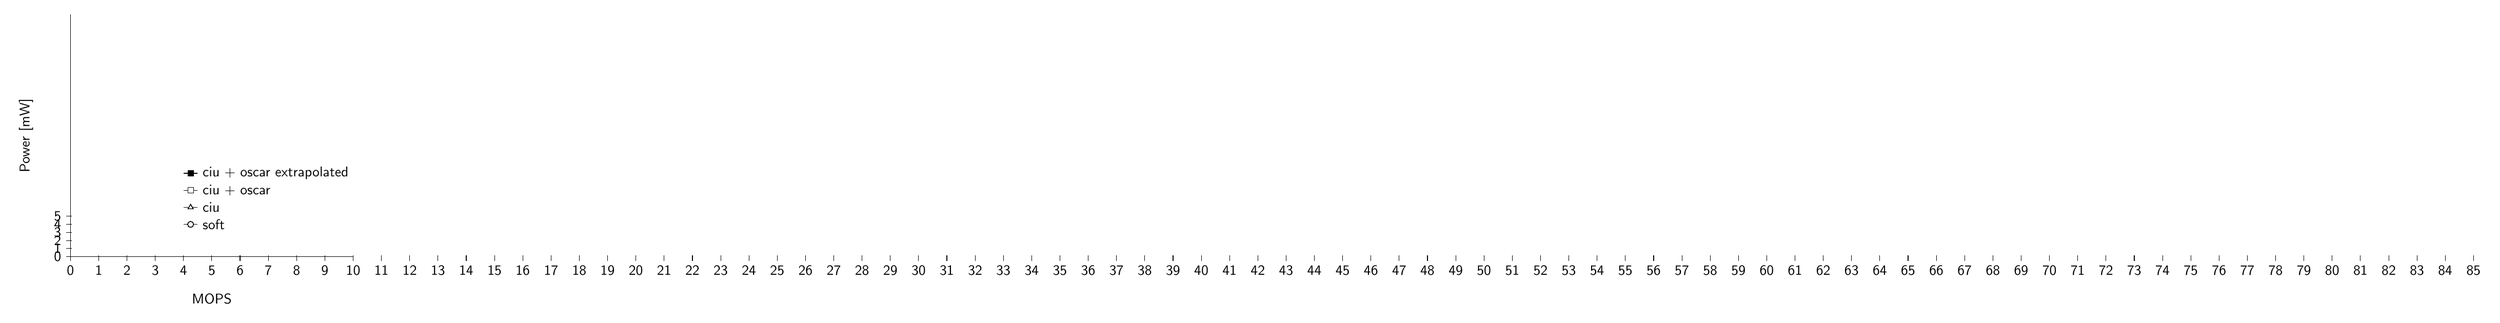
\begin{tikzpicture}[y=.2cm, x=.7cm,font=\sffamily]
 	%axis
	\draw (0,0) -- coordinate (x axis mid) (10,0);
    	\draw (0,0) -- coordinate (y axis mid) (0,30);
    	%ticks
    	\foreach \x in {0,...,85}
     		\draw (\x,1pt) -- (\x,-3pt)
			node[anchor=north] {\x};
    	\foreach \y in {0,1,...,5}
     		\draw (1pt,\y) -- (-3pt,\y) 
     			node[anchor=east] {\y}; 
	%labels      
	\node[below=0.8cm] at (x axis mid) {MOPS};
	\node[rotate=90, above=0.8cm] at (y axis mid) {Power [mW]};

	%plots
	\draw plot[mark=*, mark options={fill=white}] 
		file {plotdata/cbmc-time.dat};
	%\draw plot[mark=triangle*, mark options={fill=white} ] 
	%	file {div_ciu.dat};
	%\draw plot[mark=square*, mark options={fill=white}]
	%	file {div_ciu_oscar.dat};
	%\draw plot[mark=square*]
	%	file {div_ciu_oscar_extrapolated.dat};  
    
	%legend
	\begin{scope}[shift={(4,4)}] 
	\draw (0,0) -- 
		plot[mark=*, mark options={fill=white}] (0.25,0) -- (0.5,0) 
		node[right]{soft};
	\draw[yshift=\baselineskip] (0,0) -- 
		plot[mark=triangle*, mark options={fill=white}] (0.25,0) -- (0.5,0)
		node[right]{ciu};
	\draw[yshift=2\baselineskip] (0,0) -- 
		plot[mark=square*, mark options={fill=white}] (0.25,0) -- (0.5,0)
		node[right]{ciu + oscar};
	\draw[yshift=3\baselineskip] (0,0) -- 
		plot[mark=square*, mark options={fill=black}] (0.25,0) -- (0.5,0)
		node[right]{ciu + oscar extrapolated};
	\end{scope}
\end{tikzpicture}
\caption{\label{fig:results}
Comparison between SAT-based BMC and ACDLP: number of decisions and propagations}
\end{figure}

%
\noindent \textbf{ACDLP versus CBMC}
Fig.~\ref{fig:results} presents a comparison of the analyses using CBMC
and ACDLP.  Fig.~\ref{fig:results}(a) clearly shows that the SAT based analysis 
made significantly more decisions compared to ACDLP for all the benchmarks. 
The points on the extreme right below the diagonal in
Fig.~\ref{fig:results}(b) show that the number of propagations in the SAT based 
analysis is maximal for benchmarks that exhibit relational behaviour.  These
benchmarks are solved by octagon domain in ACDLP.  We see a reduction of at 
least two order of magnitude in the total number of decisions, propagations 
and conflicts compared to analysis using CBMC.  

Out of 85 benchmarks, SAT based analysis could prove only 26
benchmarks without any restarts.  The solver was restarted in the other 59 
cases to avoid spending too much time in ``hopeless'' branches.  By contrast, 
ACDLP solved all 85 benchmarks without restarts.  
The runtime comparison between ACDLP and CBMC are shown in 
Figure~\ref{fig:runtimes}.  ACDLP is~1.5X faster than CBMC. 
The superior performance of ACDLP is attributed to the decision heuristics, 
which exploit the high-level structure of the program, combined with the 
precise deduction by multi-way transformer and stronger learnt clause aided 
by the richer abstract domains. 
%


\noindent \textbf{ACDLP versus Astr{\'e}e}
%
To enable precise analysis using Astr{\'e}e, we manually instrument 
the benchmarks with partition directives \texttt{\_\_ASTREE\_partition\_control} 
at various control-flow joins.  These directives provides external hint to
Astr{\'e}e to guide its internal trace partition domain. 
Figure~\ref{fig:runtimes} demonstrates that Astr{\'e}e is~2X faster 
than ACDLP for {37}\% cases (32 out of 85); but the analysis using 
Astr{\'e}e shows a high degree of imprecision (marked as timeout in 
Figure~\ref{fig:runtimes}).  Astr{\'e}e reported~53 false alarms 
among~85 benchmarks.  Whereas, analysis using ACDLP produce correct 
results for all benchmarks.  Clearly, ACDLP has higher precision than 
Astr{\'e}e. Detailed analysis of the comparison between ACDLP and 
Astr{\'e}e is presented in Table~\ref{ai-result} of 
Appendix~\ref{appendix:extended_result}.  Statistics for each phase of ACDLP 
algorithm are given in Table~\ref{detailed_result} in Appendix~\ref{appendix:extended_result}.  


Our experimental evaluation suggest that ACDLP can be seen as a
technique to improve the efficiency of SAT-based BMC.  Additionally, ACDLP can
also be perceived as an automatic way to improve the precision of conventional
abstract interpretation over non-distributive lattices through automatic partition 
generation techniques such as decisions and transformer learning.

%===============================================================================

%===============================================================================
\section{Related Work}
%
The work of~\cite{franzle} presents a tight integration of SAT solving
with interval based arithmetic constraint solving to handle large constraint
systems. 
%
Silva et al.~\cite{sas12} present an abstract interpretation account of 
satisfiability algorithms derived from DPLL procedures.  
%
The work of~\cite{tacas12} is a very early instantiation of abstract 
CDCL~\cite{sas12} as an interval-based decision procedure for programs, 
but in a purely logical settings.  
%
A similar technique that lifts DPLL(T) to programs is Satisfiability Modulo 
Path Programs (SMPP)~\cite{SMPP}. SMPP enumerates program paths using a SAT 
formula, which are then verified using abstract interpretation.  
%
%The work of \cite{DBLP:conf/esop/MineBR16} proposes an algorithm inspired by 
%constraint solvers for inferring disjunctive invariants using intervals.
%
The lifting of CDCL to first-order theories is proposed
in~\cite{dpll,ndsmt,vmcai13}.
%
\Omit{ operates on a fixed first-order partial assignment lattice
  structure, where first-order variables are mapped to domain values,
  similar to constants lattice in program analysis.  } 
  More recently, ~\cite{cade17} proposed a calculus for extending theory of
  finite sets to theory of finite relations in CVC4 solver, which allows
  relational constraint solving in SMT.  
  \Omit{Unlike previous work that operates on a fixed first-order lattice,
  ACDLP can be instantiated with different abstract domains as well as product
  domains.  
  This involves model search and learning in abstract lattices.  A similar
  technique that lifts decisions, propagations and learning to theory variables
  is Model-Constructing Satisfiability Calculus (mcSAT)~\cite{vmcai13}.}
  
  ACDLP is not, however, similar to abstraction refinement. ACDLP works on a fixed
  abstraction. Also, transformer learning in ACDLP does not soundly over-approximate
  the existing program transformers. Hence, transformer learning in ACDLP is
  distinct from transformer refinement in classical CEGAR. 

\Omit { The
  abstract lattice in natural domain SMT does not have complementable
  meet irreducibles, and therefore does not support generalized clause
  learning~\cite{sas}.  On the other hand, most abstract lattice have
  complementation property, thus enabling ACDCL to perform generalized
  clause learning.  } 
%
%\cite{DBLP:journals/fmsd/BrainDGHK14} presents a similar decision and learning
%based approach for heap-manipulating programs, but uses a simplistic conflict analysis.
%
%\cite{DBLP:conf/vmcai/PelleauMTB13} describes a constraint solving algorithm
%using relational numerical domains, but performs model search only.
%
%
% is presented in . They
%use a relational domain, but focus on the model search, whereas the
%conflict analysis is simplistic and restarts the algorithm with the
%learnt clause instead of backtracking.
%}


%===============================================================================

%===============================================================================
\section{Conclusions}
In this paper, we present a general algorithmic framework for lifting 
the model search and conflict analysis procedures in satisfiability 
solvers to program analysis.  We embody these techniques in a tool, ACDLP,  
for automatic bounded safety verification of C programs over a template 
polyhedra abstract domains.  

We present an {\em abstract model search} procedure that uses a 
parameterised abstract transformer to flexibly control the precision and 
efficiency of the deductions in the template polyhedra abstract domain. 
The underlying expressivity of the abstract domain helps our decision 
heuristics to exploit the high-level structure of the program for making 
effective decisions.  The {\em abstract conflict analysis} procedure learns 
abstract transformers over a given template following a UIP computation.
Experimental evaluation over a range of benchmarks shows~10X
reduction in the total number of {\em decisions}, {\em propagations}, 
{\em conflicts} and {\em backtracking} iterations compared to CBMC.  Moreover, 
ACDLP is \rmcmt{?X} faster than CBMC.  Compared to Astr{\'e}e, ACDLP is
\rmcmt{70\%} more precise on our benchmark suite.  \rmcmt{In the future, we plan to
extend our framework to unbounded verification through invariant generation.} 


%able to exploit the expressivity of richer abstract domains 
%as well as the precision of the CDCL architecture.  \tmcmt{I don't understand this ``as well as'' business. Do we mean ``without giving up the precision of...''?}
%\Omit{
%The ACDLP analyses in this paper perform bounded model checking. Since we use abstract 
%domains, however, we will be able to extend it to unbounded verification, a possibility 
%we intend to explore in future work.
%}

%===============================================================================
%\newpage
\bibliographystyle{splncs03}
\bibliography{biblio.bib}

\newpage
\appendix
\section*{Appendix}
%
\section{Detailed Experimental Results}\label{appendix:extended_result}
\rmcmt{recount total benchmarks in tables}
Table~\ref{detailed_result} gives a detailed comparison between CBMC version
5.5 and ACDLP.  Columns~1--4 in Table~\ref{detailed_result} contain the
name of the tool, the benchmark category, the number of lines of code (LOC),
and the total number of safe and unsafe benchmarks in the respective
categories (labelled as safe/unsafe).  The solver statistics ({\em
Decisions, Propagations, Conflicts, Conflict Literals, Restarts}) per
category for CBMC and ACDLP are in columns~5--9.
%
%Column~10 reports the total time for verification per category.  

We divide the benchmarks into separate categories. 
We label the benchmarks in bit-vector regression category in SV-COMP'16 
as {\em Bit-vector}, C models of hardware circuits auto-generated by v2c 
tool as {\em Verilog-C} and hand-crafted benchmarks as {\em Control-Flow} 
category.  The total number of benchmarks in {\em bit-vector} category are 13, 
{\em Control-Flow} category contains 55 benchmarks and 
{\em Verilog-C} category has 10 benchmarks. The timeout for our
experiments is set to one hour.  All times in Table~\ref{detailed_result} 
and Table~\ref{ai-result} are in seconds. 

The benchmarks in Bit-vector category are derived from bit-vector regression
category in SV-COMP'16.  This categoty contains a total of six safe
benchmarks and~seven unsafe benchmarks.  The benchmarks in the control-flow
category vary from simple bounded loop analysis and implementation of
arithmetic operations to more complex checking for relational properties in
nested loops.  Out of~55 benchmarks in this category, 38 are safe and 17 are
unsafe.  We verified a total of ten hardware benchmarks, which are given in
Verilog.  Out of those ten benchmarks, five are safe and the remaining five
are unsafe.  The software models (in C) for the Verilog circuits are
obtained via a Verilog to C translator tool, {\em v2c}.  These software
models are then fed to CBMC and ACDLP.  The hardware benchmarks include an
implementation of a Instruction buffer logic, FIFO arbiter, traffic light
controller, cache coherence protocol, Dekker's mutual exclusion algorithm
among others.  The largest benchmark is the cache coherence protocol which
consists of~890 LOC and the smallest benchmark is TicTacToe with~67 LOC. 
The software models of these Verilog circuits uses several complex bit-wise
logic to map hardware operations into an equivalent C syntax.  It is worth
emphasizing that our abstract domain implementation can automatically handle
bit-wise operations out-of-the-box.
%
\begin{table}[!b]
\begin{center}
{
\begin{tabular}{l|l|r|r|r|r|r|r|r}
\hline
           &          &     & Safe/  &           & Propa-  &           & Conflict &          \\
  Verifier & Category & LOC & Unsafe & Decisions & gations & Conflicts & literals & Restarts \\ \hline
  CBMC & \multirow{2}{*}{Bit-vector} & \multirow{2}{*}{501} &
  \multirow{2}{*}{6/7} & 1011 & 1190 & 0 & 0 & 7 \\
  ACDLP & & & & 0 & 44 & 0 & 0 & 0 \\ \hline
  CBMC & \multirow{2}{*}{Control-Flow} & \multirow{2}{*}{692} & 
  \multirow{2}{*}{38/17} & 29382 & 379727 & 4520 & 37160 & 62 \\ 
  ACDLP & & & & 414 & 6487 & 195 & 180 & 0  \\ \hline
  CBMC & \multirow{2}{*}{Verilog-C} & \multirow{2}{*}{2422} & 
  \multirow{2}{*}{5/5} & 131932 & 322707 & 69 & 349 & 6 \\ 
  ACDLP & & & & 625 & 8196 & 22 & 22 & 0 \\ \hline
  %CBMC & \multirow{2}{*}{Numerical} & \multirow{2}{*}{} & 
  %\multirow{2}{*}{} & & & & & & \\
  %ACDLP & & & & 161 & 3130 & 10 & 5 & 0 & \\ \hline  
\end{tabular}
}
\end{center}
\caption{CBMC versus ACDLP}
\label{detailed_result}
\end{table}
%
The statistics reported in Table~\ref{detailed_result} for ACDLP is obtained 
with an ordered decision heuristic, multi-way propagation heuristic and a
first-UIP learning heuristic.  Note that the deductions using a 
multi-way heuristic are more precise than the forward or backward 
heuristics, but it takes longer time to reach the fixed-point.
Another advantage of multi-way heuristic is that it significantly 
reduces the overall number of decisions and learning iterations due to stronger 
and more precise deductions.  Analysis using ACDLP reduces the total number of 
decisions, propagations and learning compared to CBMC by a factor of~2X.  
%
\begin{table}[t]
\begin{center}
{
\begin{tabular}{l|l|r|r|r}
\hline
  Verifier & Category & \#Proved (safe/unsafe) & \#Inconclusive & \#False Positives \\ \hline
  Astr{\'e}e & \multirow{2}{*}{Bit-vector} & 5/7 & 0 & 1 \\
  ACDLP & & 6/7 & 0 & 0 \\ \hline
  Aste{\'e}e & \multirow{2}{*}{Control-Flow} & 24/9 & 0 & 22 \\
  ACDLP & & 35/17 & 3 & 0 \\ \hline
  Astr{\'e}e & \multirow{2}{*}{Verilog-C} & 2/4 & 0 & 4 \\
  ACDLP & & 4/5 & 1 & 0 \\ \hline
  %Astr{\'e}e & \multirow{2}{*}{Numerical(13)} & 6/7 &  & \\
  %ACDLP & & & & \\ \hline
\end{tabular}
}
\end{center}
  \caption{Astr{\'e}e versus ACDLP}
\label{ai-result}
\end{table}
%
Table~\ref{ai-result} gives a detailed comparison between Astr{\'e}e and
ACDLP.  Columns~1--5 in Table~\ref{ai-result} contain the name of the
tool, the benchmark category, the total number of instances proved safe or
unsafe (labelled as safe/unsafe), the total number of inconclusive
benchmarks and total number of false positives per category.

To enable precise analysis using Astr{\'e}e, we manually instrumented 
partition directives in some benchmarks.  These directives provides 
external hint to the tool to guide the trace partitioning heuristics.  
Note that it requires significant domain knowledge to select the right 
partition directive.  Usually, such high-precision is not needed for 
static analysis, since it makes the analysis very expensive.  Without 
trace partitioning, the analysis using Astr{\'e}e shows high degree of 
imprecision. 

Table~\ref{ai-result} shows that ACDLP proved more benchmarks than
Astr{\'e}e in all categories.  The total number of inconclusive results in
ACDLP is three.  The inconclusive results is because of timeout.  By
contrast, Astr{\'e}e reports a total of~27 false positives among~78
benchmarks even with manual trace partitioning.  Clearly, ACDLP is more
precise than the analysis in Astr{\'e}e.
%
%
\section{Decision Heuristics in ACDLP}
%
We have implemented several decision heuristics in ACDLP: {\em ordered}, 
{\em longest-range}, {\em random}, and the {\em Berkmin}~\cite{eugoldberg07} 
decision heuristic.  The {\em ordered} decision heuristic 
%creates an ordering among meet irreducibles, 
makes decisions on meet irreducibles that involve conditional 
variables (variables that appear in conditional branches) first 
before choosing meet irreducibles with numerical variables.  
%The ordered heuristic gives an effect of trace partitioning~\cite{toplas07}.
%
The {\em longest-range} heuristic simply keeps track of the bounds
$\numabsval_l,\numabsval_u$ of matching template rows, which are 
%\footnote{These are template rows with row vectors $\vec{c}$, $\vec{c}'$ such that $\vec{c}=-\vec{c}'$.}
row vectors $\vec{c}$, $\vec{c}'$ such that $\vec{c}=-\vec{c}'$.
%\pscmt{[that has become a bit hard to understand since some of the definitions have been removed]} 
$\numabsval_l\leq \vec{c}\vec{x}\leq \numabsval_u$, picks the one with the longest range
$\numabsval_u-\numabsval_l$, and randomly returns the meet irreducible
$\vec{c}\vec{x}\leq
\lfloor\frac{\numabsval_l+\numabsval_u}{2}\rfloor$ or its
complement. This ensures a fairness policy in selecting a variable
since it guarantees that the intervals of meet irreducibles are
uniformly restricted.
%
The {\em random} decision heuristic arbitrarily picks a meet irreducible  
for making decision. 
%
%The {\em relational} decision heuristics is only relevant for relational 
%abstract domains.  
%
The {\em Berkmin} decision heuristic is inspired by the 
decision heuristic used in the Berkmin~\cite{eugoldberg07} SAT solver.  
The Berkmin heuristic %is currently implemented for interval constraints only.  
%The heuristic 
keeps track of the activity of %an interval 
meet irreducibles that participate in conflict clauses. 
Based on the most active meet irreducible, ranges are split 
similar to the {\em longest-range} heuristic.
%
\section{Comparison of Solving Statistics in ACDLP}
%

%%%%%%%%%%%%%%%%%%%%%%%%%%%%%%%%%%%%%%%%%%%%%%%%%%%%%%%%%%%%%%%%%%%%%%%%%%%%%%%%
\begin{figure}[t]
\begin{tabular}{@{\hspace{-1.5em}}c@{\hspace{1em}}c}
\begin{tikzpicture}[scale=0.75]
	\begin{loglogaxis} [
      xmin=0.1,xmax=2500, ymin=0.1, ymax=2500, 
      xlabel=Forward Propagation, ylabel=Multi-way Propagation, 
      title={Performance of Propagation Heuristics},
			legend pos = north west,
			%legend style={at={(0.8,0.15)},
			%anchor=north,legend columns=-1 },
			]
\addplot [mark size=1pt,only marks,scatter,point meta=explicit symbolic,
	scatter/classes={s={mark=square},u={mark=triangle*,blue}},] 
	table [meta=label] {plotdata/scatter-chaotic-forward.dat};
	\legend{Safe,Unsafe}
  \addplot [domain=.1:2500] {x};
\end{loglogaxis}
\end{tikzpicture}
 &
\begin{tikzpicture}[scale=0.75]
\pgfplotscreateplotcyclelist{markstyles}{%
mark=diamond\\%
mark=square*,red\\%
mark=triangle*,blue\\%
}
	\begin{axis} [
  title={Performance of Decision Heuristics}, ymode = log,
  xmin=0, xmax=70, only marks,
  ymin=0, ymax=1600, 
  xlabel={Benchmarks},
  ylabel={time (in seconds)},
  xtick={},
  ytick={}, %{0, 0.5, 1.0, 10, 50, 100, 200, 500, 700, 1000, 1500},
	legend pos=north west, mark size=1pt, cycle list name=markstyles,
 ]
 \addplot table[x=benchmark,y=time] {plotdata/berkmin.dat};
 \addplot table[x=benchmark,y=time] {plotdata/random.dat};
 \addplot table[x=benchmark,y=time] {plotdata/ordered.dat};
 \addlegendentry{Berkmin}
 \addlegendentry{Random}
 \addlegendentry{Ordered}
 %\addplot [domain=.1:2500] {};
 \end{axis}
\end{tikzpicture} \\
(a) & (b)
\end{tabular}
\caption{\label{prop-dec}
Effect of Propagation Heuristics and Decision Heuristics in ACDLP
}
\end{figure}
%%%%%%%%%%%%%%%%%%%%%%%%%%%%%%%%%%%%%%%%%%%%%%%%%%%%%%%%%%%%%%%%

%
\paragraph{Propagation Strategy.}
%
Fig.~\ref{prop-dec}(a) presents a comparison between the {\em forward}
propagation strategy and the {\em multi-way} propagation strategy in ACDLP.  The
choice of strategy influences the total number of decisions
and clause learning iterations.  Hence, the propagation strategy has a
significant influence on the runtime, which can be seen in
Fig.~\ref{prop-dec}(a).  Compared to forward propagation, the multi-way
strategy may take more iterations to reach the fixed-point, but it
significantly reduces the number of decisions and conflicts, in
particular for the unsafe benchmarks.  This is attributed to the higher
precision of the meet irreducibles inferred by the multi-way strategy, which
subsequently aids the decision heuristics to make better decisions.

\paragraph{Decision Heuristics.}
%
Fig.~\ref{prop-dec}(b) shows the performance of different decision
heuristics in ACDLP.  Note that the runtimes for all decision heuristics are
obtained with the multi-way propagation strategy.  The runtimes are very
close, but we can still discern some key characteristics of these
heuristics.  The Berkmin heuristic performs consistently well for most safe
benchmarks and all bit-vector category benchmarks.  By contrast, the ordered
heuristic performs better for programs with conditional branches since it
prioritises decisions on meet irreducibles that appear in conditionals.  The
runtimes for the random heuristic are marginally higher than for the other
two.  This suggests that domain-specific decision heuristics are important
for ACDLP.
%
%\tmcmt{I don't see any such conclusion can be reached from the
%graph shown. It looks, at least at this scale, like it really doesnt matter which
%heuristic is used! And if RANDOM is best, well this contradicts the last sentence, doesn't it?}

\Omit{
Whereas activity-based heuristics such as Berkmin heuristic which 
works well in propositional cases performs best for benchmarks 
that encountered the maximum number of conflicts to prove safety, 
thus allowing the heuristics to choose the decision variable among the set of learnt clauses.   
}

\paragraph{Learning.}
%
Learning has a significant influence on the runtime of ACDLP.  We compare
the UIP-based learning technique with an analysis that performs classical 
DPLL-style analysis~\cite{DPLL62}.
%chronoligical backtracking without learning.  
The effect of UIP computation allows ACDLP to backtrack non-chronologically 
and guide the model search with a learnt transformer.  But classical 
DPLL-style analysis exhibits case-enumeration behaviour and could not finish 
within the time bound for 20\% of our benchmarks.
%
\section{Computing Lazy Closure in Template Polyhedra Domain}\label{appendix:lazyclosure}
%
Computing the closure for relational domains, such as octagons, is
expensive~\cite{pldi15}.  An~advantage of our formalism in
Eq.~(\ref{eq:at2}) is that the \emph{closure} operation for relational
domains can be computed in a lazy manner through the construction of a
subdomain.  A subdomain $\subdomain$ is constructed from domain $\domain$
for a abstract deduction transformer $\abstransel{\subdomain}$, such that
$\subdomain=\makesubdomain_\domain(\subvars)$, where $\subvars$ are
variables that appears in $\abstransel{\subdomain}$.  The construction of
$\subdomain$ allows us to perform one step of the closure operation when
$\abstransel{\subdomain}$ is applied.
%
For example, let us consider $\domain=\octagons[\{x,y,z\}]$ and
$\subvars=\{y\}$. An octagonal inequality relates at 
most two variables. Thus it is sufficient to consider the subdomain
$\makesubdomain_\domain(\{y\})=\octagons[\{y\}]\cup\octagons[\{x,y\}]\cup\octagons[\{y,z\}]$,
which will compute the one-step transitive relations of~$y$ with each
of the other variables. 
%
Only if a abstract deduction transformer subsequently makes new deductions 
on $x$ or $z$, then the next step of the closure will be computed through 
the subdomain $\octagons[\{x,z\}]$.
\Omit{
Hence, when the abstract deduction transformer is applied we do not
compute the full closure in the full domain,
but we compute only a single step of the closure in a restricted
domain, which makes single deduction steps more efficient.
}
Hence, an application of abstract deduction transformer does not 
compute the full closure in the full domain, but compute only a 
single step of the closure in a restricted domain, which makes each 
deduction step more efficient.  Thus, we delay the closure operation 
until the point where it is absolutely necessary.  
%This makes our deductions in relational domain more efficient.  
%

Let us demonstrate the idea of lazy closure with a concrete example.  Assume
the program in the left of Figure~\ref{fig:lazy}.  The corresponding
locations are marked as L1, L2.  We~analyze the program with an octagon
domain ($\octagons$), which computes the closure in lazy manner.  The lazy
closure computation in octagon domain is shown in the right of
Figure~\ref{fig:lazy}.

Recall that a closure in octagon domain achieves a normal form by computing all
implied constraints among numerical variables. The closure operation is 
necessary to perform precise domain operations.  The ACDLP analysis in
Figure~\ref{fig:lazy} performs forward propagation in $\octagons$ by creating a 
subdomain $\subdomain$ for every transformer using the function $\makesubdomain$.  
Note that the choice of subdomain over lhs variables of the transformers guides the 
analysis in forward direction in this example. The subdomain 
corresponding to L1 over $y$ is given by 
$\octagons[\{y\}]\cup\octagons[\{y,z\}]$.  This means, only those deductions 
which are implied by the domain $\octagons[\{y\}]\cup\octagons[\{y,z\}]$ can be
inferred at L1.  No deductions over $\octagons[\{y,x\}]$ is performed at L1.  
Thus, we delay the deductions over $\{y,x\}$ until we encounter an abstract 
transformer over these variables.  This does not admit a normal form for 
octagonal constraints after the application of the transformer at L1, but it 
makes the deduction step at L1 more efficient.  

Assume that the initial abstract value $(\absval)$ is $\absval=(x=y)$. 
Then, the deduction at L1 infers ${y=z}$.  Thus, the updated abstract value
is $\absval=\{x=y \wedge y=z\}$.  We now analyze the transformer at L2.  The
subdomain for L2 over variable $x$ (for forward propagation) is given by
$\octagons[\{x\}]\cup\octagons[\{x,y\}]\cup\octagons[\{x,z\}]\cup\octagons[\{x,w\}]$. 
Note that we delayed the deduction over $\octagons[\{x,y\}]$ at L1, but only
perform the deductions over $\octagons[\{x,y\}]$ at L2.  This is the notion
of lazy closure computation.  The new deductions at L2 are $\{x=z, x-w \leq
1, x-w \geq 1\}$ and the final abstract value is $\absval=\{x=y
\wedge\allowbreak y=z \wedge\allowbreak x=z \wedge\allowbreak x-w \leq 1
\wedge x-w \geq 1\}$.  Thus, the normal form over $\octagons{\{x,y,z\}}$ is
only achieved at L2.  However, we do not perform deductions over
$\octagons{\{w,z\}}$ at L2, which is delayed until the point where we
encounter an abstract transformer that forces us to infer such deductions.
%
\begin{figure}[htbp]
\centering
\begin{tabular}{c|c}
\hline
C program & Lazy Closure Computation \\
\hline
\scriptsize
\begin{lstlisting}[mathescape=true,language=C]
int main() {
  L1: y=z;
  L2: x=w+1;
}
\end{lstlisting}
&
\begin{lstlisting}[mathescape=true,language=C]
L1: $\makesubdomain_\domain(\{y\})=\octagons[\{y\}]\cup\octagons[\{y,z\}]$
    New Deductions: $\{y=z\}$
    Abstract Value: $\absval=\{x=y \wedge y=z\}$
L2: $\makesubdomain_\domain(\{x\})=\octagons[\{x\}]\cup\octagons[\{x,y\}]\cup\octagons[\{x,z\}]\cup\octagons[\{x,w\}]$
    New Deductions: $\{x=z, x-w \leq 1, x-w \geq 1\}$
    Abstract Value: $\absval=\{x=y \wedge y=z \wedge x=z \wedge x-w \leq 1 \wedge x-w \geq 1\}$
\end{lstlisting}
\\
\hline
\end{tabular}
\caption{\label{fig:lazy}
C Program and Lazy closure operation for Octagons}
\end{figure}
%
\section{Difference between ACDLP and CEGAR}
%
ACDLP is not, however, similar to abstraction refinement. ACDLP works on a fixed abstraction.  
Also, transformer learning in ACDLP does not soundly over-approximate the existing program 
transformers, hence it is distinct from transformer refinement in classical Counterexample 
Guided Abstraction Refinement (CEGAR).
%
%===============================================================================
\section{Gamma Complete Procedure in ACDLP}
\Omit{
The termination criterion of CDCL algorithm checks 
whether all variables in the CNF formula have been assigned, 
in which case the algorithm terminates indicating that the 
CNF formula is satisfiable~\cite{cdcl}. An alternative 
termination criterion is to check whether all clauses 
are satisfied.  However, modern CDCL based SAT solvers checks 
whether all the variables in the formula are assigned since the 
clause state can not be maintained accurately~\cite{cdcl}.
}

Recall that an over-approximating abstract transformer 
$f_{o}$ of a transformer $f$ is $\gamma$-complete with 
respect to an abstract element $a$ if $\gamma \circ f_{o}(a) = f \circ \gamma(a)$.  

If every transformer $f_{o}$ in $\varphi$ is $\gamma$-complete and 
produces a singleton value in the concrete, then ACDLP terminates 
with a satisfying assignment.  However, it is expensive to check whether all
$f_o$ are $\gamma$-complete.  An alternative is to check whether 
all program variables are assigned singleton values following the least fixed 
point computation in the propagation phase.  This corresponds to the 
termination condition in a SAT solver which checks whether all variables 
in the CNF formula have been assigned.

We present a more sophisticated $\gamma$-complete procedure in ACDLP based 
on a technique called {\em partial evaluation}.  A decision in ACDLP 
may render some $f_o \in \varphi$ vacuously true, for example, decisions on 
conditional branch predicates.  We call such decision, {\em choice decision}.
The core idea of partial evaluation technique is based on the fact 
that the variables appearing in non-vacuous $f_o$ can only contribute to 
determining the satisfiability of $\varphi$ following a choice decision. 
We call these variables {\em sensitive variables} $(V_s)$ and the rest 
{\em don't care variables} $(V_d)$.  Therefore, assignments to sensitive 
variables are sufficient to infer the truth of $\varphi$.  If $\varphi$ is 
{\em true}, then the abstract value obtained from the deductions via choice 
decision and sensitive variables produces a satisfying assignment for $\varphi$, 
and hence a counterexample. 

\Omit{
The partial evaluation technique identifies all non-singleton variables that 
do not contribute to a feasible path from a choice decision. We call these variables 
{\em don't care variables} for the current choice decision.  The don't care variables 
are identified via path-sensitive analysis that computes analysis information based on 
the predicates at conditional branch instructions. 
}

We explain the partial evaluation technique through don't care 
variables with a simple example.  Consider the program in 
Figure~\ref{fig:gc-example}. The second column of 
Figure~\ref{fig:gc-example} shows the corresponding SSA. 
The program is unsafe. The unsafe trace is shown in bold in third 
column of figure~\ref{fig:gc-example}. 
%
\begin{figure}[t]
\centering
\begin{tabular}{c|c|c}
\hline
Program & SSA & Unsafe trace \\
\hline
\scriptsize
\begin{lstlisting}[mathescape=true,language=C]
 int x, y; 
 _Bool c;
 assume(0 <= x && 
       x <= 1); 
 if(c) 
  x++; 
 else 
  x--; 
 assert(x<=0); 
\end{lstlisting} 
&
\begin{lstlisting}[mathescape=true,language=C]
cond#21=(x#16 >= 0 && 
        !(x#16 >= 2))
cond#22=(c#20=true)
guard#22=(cond#21 && guard#0)
x#23=1+x#16
guard#23=(cond#22 && guard#22)
cond#24=true
x#25=-1 + x#16
guard#25=(!cond#22 && guard#22)
x#phi26=(guard#25?x#25:x#23)
guard#26=(cond#24 && 
         guard#23 || guard#25)
!(x#phi26 > 0)||!guard#26
\end{lstlisting}
&
\begin{minipage}{3.0cm}
\centering
%\vspace*{0.3cm}
\scalebox{.5}{\import{figures/}{example.pspdftex}}
%\caption{\label{fig:oct}}
\end{minipage}
\\
\hline
\end{tabular}
\caption{\label{fig:gc-example}  C program, SSA and unsafe trace}
\end{figure}
%

Consider the SSA statement $x\#phi26 = (guard\#25 ? x\#25 : x\#23)$, shown in 
column~2 of Figure~\ref{fig:gc-example}. A CNF representation of the SSA 
statement is given by, 
$(!(guard\#25) \vee (x\#phi26=x\#25)) \wedge ((guard\#25) \vee (x\#phi26=x\#23))$. 
Let $C1=(!(guard\#25) \vee (x\#phi26 = x\#25))$ and $C2=((guard\#25) \vee
(x\#phi26=x\#23))$. 
Assume that we make a choice decision, $cond\#22=true$. This subsequently 
infers that $guard\#25=false$ which makes the clause $C1$ vacuously true. Hence, 
ACDLP only needs to evaluate the truth of $(x\#phi26=x\#23)$ in $C2$. 
Thus, the variable $x\#25$ is don't care variable since it belongs to the 
vacuous clause $C1$ obtained from the choice decision for conditional 
predicate $cond\#22=true$.  The set of sensitive variables are 
$\{x\#23, x\#phi26\}$.

When the don't care variables has already been identified, then ACDLP simply 
restricts the decisions to the {\em sensitive} variables.  We implemented a 
specific decision heuristic called {\em singleton decision heuristic} that 
explicitly assigns singleton values to these {\em sensitive variables}.  
For our example, ACDLP makes a decision 
on the interval of $x\#23 = [1,2]$, say $x\#23=1$, followed by the propagation 
which immediately infers that the program is unsafe.  ACDLP then terminates
and returns a satisfying assignment to $\varphi$ that contains concrete 
assignments to the sensitive variables only.

However, if the assignment to the sensitive variables does not satisfy 
$\varphi$, then ACDLP undoes all the deductions made from the singleton 
assignments to the sensitive variables and backtracks up to the point where 
the choice decision was made. 

\Omit{
The advantages of our proposed gamma-complete procedure are two folds. 
\begin{enumerate}
  \item It intelligently identifies the set of sensitive program variables through a 
choice decision thereby restricting future decisions on these variables.  
  \item It may terminate with a satisfying assignment (or counterexample trace) even 
when all variables in the program are not assigned, thereby leading to faster 
counterexample detection.
\end{enumerate}

%\section{Gamma Complete Procedure}
\begin{algorithm2e}
\DontPrintSemicolon
\SetKw{return}{return}
\SetKw{continue}{continue}
\SetKwRepeat{Do}{do}{while}
\SetKwData{conflict}{conflict}
\SetKwData{safe}{safe}
\SetKwData{sat}{sat}
\SetKwData{unsafe}{unsafe}
\SetKwData{unknown}{unknown}
\SetKwData{true}{true}
\SetKwData{false}{false}
\SetKwInOut{Input}{input}
\SetKwInOut{Output}{output}
\SetKwFor{Loop}{Loop}{}{}
\SetKw{KwNot}{not}
  \Input{Abstract value $\absval$ and set of sensitive variables $V_s$}
  \Output{\true if $\absval$ is gamma complete, else \false}
  \ForEach{$m \in \decomp(\absval)$}{
    \uIf{$vars(m) \in V_s$} {
      \uIf{$val(m, \absval)$ is singleton} {
        \continue
      }
      \uElse {
         \return \false \;
      }
    }
    \uElse {
      \continue 
    }
  }
  \return \true \;
\caption{Gamma Complete procedure $gammaComplete(\absval, V_s)$
  \label{Alg:gammacomplete}}
\end{algorithm2e}
%
Algorithm~\ref{Alg:gammacomplete} presents the gamma complete procedure that
checks whether a given abstract value $\absval$ is gamma complete with respect
to the given set of sensitive variables $V_s$. Note that the set $V_s$ is
obtained from the least fixed point computation in the deduction phase.  The
procedure $vars(m)$ returns the variables involved in the meet irreducibles $m$.
For example, $vars(x<10)$ returns $x$.  The procedure $val(m, \absval)$ returns 
the upper bound and the lower bound of a meet irreducible $m$ with respect to
the abstract value $\absval$.  For example, $val(x>5, x>5 \wedge y>10 \wedge x<10)$  
returns the interval $x=[6,9]$.  The procedure $vars()$ and $val()$ are domain
operations. 
}
%
\Omit{
\begin{mytheorem}
  (Soundness). Given a choice decision $d$, let $V_s$ be the set of sensitive 
  variables and $a$ be the abstract value obtained from deductions
  through $V_s$ and $d$. If $gammaComplete(a,V_s)$ returns {\em true}, then 
  $\varphi$ is satisfiable, and ACDLP terminates with the counterexample trace $a$.
\end{mytheorem}
}
%

%===============================================================================
%
\section{Program and Property Driven Trace partitioning in ACDLP}
ACDLP performs automatic program and property driven trace partitioning. 
This is illustrated with an example in Figure~\ref{fig:tp}. Consider a 
simple program $P$ in left side of Figure~\ref{fig:tp}.  A simple forward 
interval analysis cannot prove safety of $P$ due to control-flow join 
following the if-else branch.  However, the analysis using ACDLP makes a decision 
on the variable $\langle y: [-\inf, 3] \rangle$ which implicitly constructs
a trace partitioning, as shown in right-hand side of Figure~\ref{fig:tp}. 
Interval analysis using above decision immediately leads to safety.  At 
this point, the analysis backtracks, discarding all propagations that leads to conflict, 
and learns that $\langle y: [4, +\inf] \rangle$.  Interval analysis also proves that 
$P$ is safe with the learnt clause.  The analysis cannot backtrack further and 
therefore terminates, proving that the program is safe.  
% 
\begin{figure}[htbp]
\centering
\begin{tabular}{c|c}
\hline
C program & Partitioned Program \\
\hline
\scriptsize
\begin{lstlisting}[mathescape=true,language=C]
void foo(int x, int y) 
{
  if(y < 4)
   x = 1;
  else 
   x = -1;
  assert(x != 0); 
}
\end{lstlisting}
&
\begin{lstlisting}[mathescape=true,language=C]
void foo_partitioned() 
{
  if(y < 4) {
   foo(x, y);
   assert(x != 0); 
  }
  else {
    foo(x, y);
    assert(x != 0); 
  }
}
\end{lstlisting}
\\
\hline
\end{tabular}
\caption{\label{fig:tp}
C Program and its corresponding partitions}
\end{figure}
%
The above example illustrates that ACDLP automatically performs 
program and property-driven trace partitioning.  The partition is 
program dependant because if the branch condition in $P$ was $(y<10)$, 
then ACDLP would have generated a different partition, 
$\langle y: [-\infty, 9], y: [10, +\infty] \rangle$. The partition is 
property-dependant because if the assertion was $assert(x < 1)$, then 
no splitting would have been needed to prove safety. 
%
\Omit{
\section{Correspondance between Propositional CDCL and Abstract Interpretation}
%
The correspondences between propositional CDCL and lattice-based abstractions are 
shown in Table~\ref{connection}. 
\begin{table}[]
\centering
\caption{Components in propositional solver and their counterparts in
  lattice-theory}
\label{connection}
\begin{tabular}{ll}
\hline  
  Propositional Solver & Abstract Interpretation \\
\hline
Partial assignment & Abstract Domain with complementable meet irreducibles \\
Singleton assignments & Meet Irreducibles   \\
CNF formula & Abstract Deduction Transformer    \\
Unit rule & Best Abstract Transformer \\
BCP & Greatest Fixed-Point Computation \\
Decision & Dual Widening \\ 
Conflict Analysis & Abductive Reasoning \\
Clause Learning & Synthesizing Abstract Transformer for negation \\ 
\hline
\end{tabular}
\end{table}
%
\section{Abstract DPLL versus Abstract CDCL}
%
Fig.~\ref{fig:dpll} and Fig.~\ref{fig:cdcl} demonstrates the Abstract DPLL
style (ADPLL) analysis and Abstract CDCL-style (ACDLP) analysis with
interval domain.  Figure~\ref{fig:dpll} and Figure~\ref{fig:cdcl} give a
program on the left and the result of ADPLL and ACDLP analysis on the right,
respectively.  Starting with a decision $x=[0,\infty]$, both the analysis
could not infer deductions necessary for proving safety.  Hence, it makes a
decision $y=[0,\infty]$, which also does not lead to safety.  The analysis
now makes further decisions on variable $y$, which eventually lead to a {\em
proof}.  At this point, a ADPLL-style analysis performs a case-based
reasoning, that is, try $y=[-\infty, 4]$.  However, a ACDCL-style analysis
performs a generalization step which shows that the proof is valid even when
$y=[4,\infty]$.  The ACDCL analysis learns the reason for the conflict.  It
performs deductions with the learnt clause and immediately proof safety. 
The ADPLL analysis requires a total of 14 decisions to prove safety, whereas
ACDLP analysis requires only 4 decisions to prove safety.  This demonstrates
the benefit of learning in ACDLP-style analysis over ADPLL.

\begin{figure}[t]
\centering
\begin{tabular}{c|c}
\hline
C program & DPLL with Forward Interval Analysis \\
\hline
\scriptsize
\begin{lstlisting}[mathescape=true,language=C]
int main()
{
  if(y<4)
   x=1;
  else 
   x=-1;
  assert(x!=0);
}
\end{lstlisting}
&
\begin{lstlisting}[mathescape=true,language=C]
1. x:[0,$\infty$]
2. x:[0,$\infty$], y:[0,$\infty$]
3. x:[0,$\infty$], y:[5,$\infty$] $\implies$ PROOF
4. x:[0,$\infty$], y:[-$\infty$,4]
5. x:[0,$\infty$], y:[-$\infty$,3] $\implies$ PROOF
6. x:[0,$\infty$], y:[4,4] $\implies$ PROOF
7. x:[0,$\infty$], y:[-$\infty$,0]

8. x:[-$\infty$,0]
9. x:[-$\infty$,0], y:[0,$\infty$]
10. x:[-$\infty$,0], y:[5,$\infty$] $\implies$ PROOF
11. x:[-$\infty$,0], y:[-$\infty$,4]
12. x:[-$\infty$,0], y:[-$\infty$,3] $\implies$ PROOF
13. x:[-$\infty$,0], y:[4,4] $\implies$ PROOF
14. x:[-$\infty$,0], y:[-$\infty$,0] $\implies$ PROOF
\end{lstlisting}
\\
\hline
\end{tabular}
\caption{\label{fig:dpll}
DPLL-style Analysis with Intervals}
\end{figure}

\begin{figure}[t]
\centering
\begin{tabular}{c|c}
\hline
C program & CDCL with Forward Interval Analysis \\
\hline
\scriptsize
\begin{lstlisting}[mathescape=true,language=C]
int main()
{
  if(y<4)
   x=1;
  else 
   x=-1;
  assert(x!=0);
}
\end{lstlisting}
&
\begin{lstlisting}[mathescape=true,language=C]
1. x:[0,$\infty$]
2. x:[0,$\infty$], y:[0,$\infty$]
3. x:[0,$\infty$], y:[5,$\infty$] $\implies$ PROOF (Generalize y)
5. x:[0,$\infty$], y:[4,$\infty$] $\implies$ PROOF (Learn)
6. x:[0,$\infty$], y:[-$\infty$,3] $\implies$ PROOF
\end{lstlisting}
\\
\hline
\end{tabular}
\caption{\label{fig:cdcl}
CDCL-style Analysis with Intervals}
\end{figure}
}

%
\Omit{
\section{Octagon Analysis in ACDCL}
\rmcmt{correct the constraints}
\begin{figure}[t]
\centering
\begin{tabular}{c|c}
\hline
C program & Forward Octagon Analysis \\
\hline
\scriptsize
\begin{lstlisting}[mathescape=true,language=C]
int main()
{
  L0:int x,y,z,d,g;
  L1:assume(x==y || x==-y);
  L2:if(x<0)  d=-x;
  L3:else     d=x;  
  L4:if(y<0)  g=-y;
  L5:else     g=y;
  L6:z = d-g;    
  L7:assert(z==0);
}
\end{lstlisting}
&
\begin{lstlisting}[mathescape=true,language=C]
L1: [$\top$]
L2: [d-1>=0; d+x>=0; -d-x>=0; d-x-2>=0; -x-1>=0]
L3: [d>=0; -d+x>=0; d+x>=0; x>=0; d-x>=0]
L4: [d>=0; d+g-1>=0; g-1>=0; d+x>=0; d-x>=0; 
     g+y>=0; d-y-1>=0;-g-y>=0; g-y-2>=0; -y-1>=0]
L5: [d>=0; d+g>=0; g>=0; d+x>=0; d-x>=0; 
     g+y>=0; g-y>=0]
L6: [d>=0; d+g>=0; g>=0; d+x>=0; d-x>=0; 
     g+y>=0; g-y>=0; g+z>=0; d-z>=0]
L7: [$\top$]     
\end{lstlisting}
\\
\hline
\end{tabular}
\caption{\label{fig:octagon}
C Program and its corresponding forward octagon analysis}
\end{figure}
}
%
\Omit{
\section{Polyhedral Analysis with Multi-way Interval Analysis}
%
Consider the program in left of Fig.~\ref{fig:interval} 
and the corresponding standard forward interval analysis 
shown in the right.  Fig.~\ref{fig:polyhedra} shows the 
corresponding octagon and polyhedral analysis in the left and 
right side respectively. Clearly, only polyhedral analysis can 
prove safety of the program.  This is because the expression $y\leq2*x$ in the 
{\em assert} statement can only be expressed with a polyhedra 
abstract domain.  However, ACDLP with interval analysis
ACDLP can have the same precision of a standard forward polyhedral analysis 
in this case. \rmcmt{TBD}
%
\begin{figure}[t]
\centering
\begin{tabular}{c|c}
\hline
C program & Forward Interval Analysis \\
\hline
\scriptsize
\begin{lstlisting}[mathescape=true,language=C]
int main()
{
 L0:unsigned x,y,z;
 L1: assume(x>=1 && x<=5);
 L2: if(z>=0)
 L3:   y=2*x-1;
 L4:  else 
 L5:   y=2*x-2;
 L6: assert(y<=2*x);
}
\end{lstlisting}
&
\begin{lstlisting}[mathescape=true,language=C]
L1: [x-1>=0; -x+5>=0]
L2: [x-1>=0; -x+5>=0; z>=0]
L3: [x-1>=0; -x+5>=0; y-1>=0; -y+9>=0; z>=0]
L4: [x-1>=0; -x+5>=0; -z-1>=0]
L5: [x-1>=0; -x+5>=0; y-3>=0; -y+11>=0; -z-1>=0]
L6: [x-1>=0; -x+5>=0; y-1>=0; -y+11>=0] $\implies$ [$\top$]
\end{lstlisting}
\\
\hline
\end{tabular}
\caption{\label{fig:interval}
C Program and its corresponding forward interval analysis}
\end{figure}
%
\begin{figure}[t]
\centering
\begin{tabular}{c|c}
\hline
  Forward Octagon Analysis & Forward Polyedral Analysis \\
\hline
\scriptsize
\begin{lstlisting}[mathescape=true,language=C]
L1: [x-1>=0; -x+5>=0] 
L2: [x-1>=0; -x+5>=0; 
     -x+z+5>=0; x+z-1>=0; z>=0] 
L3: [x-1>=0; -x+5>=0; -x+y>=0; 
     x+y-2>=0; y-1>=0; -x-y+14>=0; 
     x-y+4>=0; -y+9>=0; -x+z+5>=0; x+z-1>=0;
     -y+z+9>=0; y+z-1>=0; z>=0] 
L4: [x-1>=0; -x+5>=0; -x-z+4>=0; 
     x-z-2>=0; -z-1>=0]
L5: [x-1>=0; -x+5>=0; -x+y-2>=0; x+y-4>=0; 
     y-3>=0; -x-y+16>=0; x-y+6>=0; -y+11>=0; 
     -x-z+4>=0; x-z-2>=0; -y-z+10>=0; 
     y-z-4>=0; -z-1>=0]
L6:  [x-1>=0; -x+5>=0; -x+y>=0; x+y-2>=0; 
      y-1>=0; -x-y+16>=0; x-y+6>=0; -y+11>=0] 
     $\implies$ [$\top$]
\end{lstlisting}
&
\begin{lstlisting}[mathescape=true,language=C]
L1: [-x+5>=0; x-1>=0]
L2: [-x+5>=0; z>=0; x-1>=0]
L3: [-2x+y+1=0; -x+5>=0; z>=0; x-1>=0]
L4: [-x+5>=0; -z-1>=0; x-1>=0]
L5: [-2x+y-1=0; -x+5>=0; -z-1>=0; x-1>=0]
L6: [-2x+y+1>=0; -x+5>=0; x-1>=0; 2x-y+1>=0]
    $\implies$ [$\bot$]
\end{lstlisting}
\\
\hline
\end{tabular}
\caption{\label{fig:polyhedra}
C Program and its corresponding forward polyhedral analysis}
\end{figure}
}

%\extendedonly{
%\appendix
\section*{Appendix}
%
\section{Detailed Experimental Results}\label{appendix:extended_result}
\rmcmt{recount total benchmarks in tables}
Table~\ref{detailed_result} gives a detailed comparison between CBMC version
5.5 and ACDLP.  Columns~1--4 in Table~\ref{detailed_result} contain the
name of the tool, the benchmark category, the number of lines of code (LOC),
and the total number of safe and unsafe benchmarks in the respective
categories (labelled as safe/unsafe).  The solver statistics ({\em
Decisions, Propagations, Conflicts, Conflict Literals, Restarts}) per
category for CBMC and ACDLP are in columns~5--9.
%
%Column~10 reports the total time for verification per category.  

We divide the benchmarks into separate categories. 
We label the benchmarks in bit-vector regression category in SV-COMP'16 
as {\em Bit-vector}, C models of hardware circuits auto-generated by v2c 
tool as {\em Verilog-C} and hand-crafted benchmarks as {\em Control-Flow} 
category.  The total number of benchmarks in {\em bit-vector} category are 13, 
{\em Control-Flow} category contains 55 benchmarks and 
{\em Verilog-C} category has 10 benchmarks. The timeout for our
experiments is set to one hour.  All times in Table~\ref{detailed_result} 
and Table~\ref{ai-result} are in seconds. 

The benchmarks in Bit-vector category are derived from bit-vector regression
category in SV-COMP'16.  This categoty contains a total of six safe
benchmarks and~seven unsafe benchmarks.  The benchmarks in the control-flow
category vary from simple bounded loop analysis and implementation of
arithmetic operations to more complex checking for relational properties in
nested loops.  Out of~55 benchmarks in this category, 38 are safe and 17 are
unsafe.  We verified a total of ten hardware benchmarks, which are given in
Verilog.  Out of those ten benchmarks, five are safe and the remaining five
are unsafe.  The software models (in C) for the Verilog circuits are
obtained via a Verilog to C translator tool, {\em v2c}.  These software
models are then fed to CBMC and ACDLP.  The hardware benchmarks include an
implementation of a Instruction buffer logic, FIFO arbiter, traffic light
controller, cache coherence protocol, Dekker's mutual exclusion algorithm
among others.  The largest benchmark is the cache coherence protocol which
consists of~890 LOC and the smallest benchmark is TicTacToe with~67 LOC. 
The software models of these Verilog circuits uses several complex bit-wise
logic to map hardware operations into an equivalent C syntax.  It is worth
emphasizing that our abstract domain implementation can automatically handle
bit-wise operations out-of-the-box.
%
\begin{table}[!b]
\begin{center}
{
\begin{tabular}{l|l|r|r|r|r|r|r|r}
\hline
           &          &     & Safe/  &           & Propa-  &           & Conflict &          \\
  Verifier & Category & LOC & Unsafe & Decisions & gations & Conflicts & literals & Restarts \\ \hline
  CBMC & \multirow{2}{*}{Bit-vector} & \multirow{2}{*}{501} &
  \multirow{2}{*}{6/7} & 1011 & 1190 & 0 & 0 & 7 \\
  ACDLP & & & & 0 & 44 & 0 & 0 & 0 \\ \hline
  CBMC & \multirow{2}{*}{Control-Flow} & \multirow{2}{*}{692} & 
  \multirow{2}{*}{38/17} & 29382 & 379727 & 4520 & 37160 & 62 \\ 
  ACDLP & & & & 414 & 6487 & 195 & 180 & 0  \\ \hline
  CBMC & \multirow{2}{*}{Verilog-C} & \multirow{2}{*}{2422} & 
  \multirow{2}{*}{5/5} & 131932 & 322707 & 69 & 349 & 6 \\ 
  ACDLP & & & & 625 & 8196 & 22 & 22 & 0 \\ \hline
  %CBMC & \multirow{2}{*}{Numerical} & \multirow{2}{*}{} & 
  %\multirow{2}{*}{} & & & & & & \\
  %ACDLP & & & & 161 & 3130 & 10 & 5 & 0 & \\ \hline  
\end{tabular}
}
\end{center}
\caption{CBMC versus ACDLP}
\label{detailed_result}
\end{table}
%
The statistics reported in Table~\ref{detailed_result} for ACDLP is obtained 
with an ordered decision heuristic, multi-way propagation heuristic and a
first-UIP learning heuristic.  Note that the deductions using a 
multi-way heuristic are more precise than the forward or backward 
heuristics, but it takes longer time to reach the fixed-point.
Another advantage of multi-way heuristic is that it significantly 
reduces the overall number of decisions and learning iterations due to stronger 
and more precise deductions.  Analysis using ACDLP reduces the total number of 
decisions, propagations and learning compared to CBMC by a factor of~2X.  
%
\begin{table}[t]
\begin{center}
{
\begin{tabular}{l|l|r|r|r}
\hline
  Verifier & Category & \#Proved (safe/unsafe) & \#Inconclusive & \#False Positives \\ \hline
  Astr{\'e}e & \multirow{2}{*}{Bit-vector} & 5/7 & 0 & 1 \\
  ACDLP & & 6/7 & 0 & 0 \\ \hline
  Aste{\'e}e & \multirow{2}{*}{Control-Flow} & 24/9 & 0 & 22 \\
  ACDLP & & 35/17 & 3 & 0 \\ \hline
  Astr{\'e}e & \multirow{2}{*}{Verilog-C} & 2/4 & 0 & 4 \\
  ACDLP & & 4/5 & 1 & 0 \\ \hline
  %Astr{\'e}e & \multirow{2}{*}{Numerical(13)} & 6/7 &  & \\
  %ACDLP & & & & \\ \hline
\end{tabular}
}
\end{center}
  \caption{Astr{\'e}e versus ACDLP}
\label{ai-result}
\end{table}
%
Table~\ref{ai-result} gives a detailed comparison between Astr{\'e}e and
ACDLP.  Columns~1--5 in Table~\ref{ai-result} contain the name of the
tool, the benchmark category, the total number of instances proved safe or
unsafe (labelled as safe/unsafe), the total number of inconclusive
benchmarks and total number of false positives per category.

To enable precise analysis using Astr{\'e}e, we manually instrumented 
partition directives in some benchmarks.  These directives provides 
external hint to the tool to guide the trace partitioning heuristics.  
Note that it requires significant domain knowledge to select the right 
partition directive.  Usually, such high-precision is not needed for 
static analysis, since it makes the analysis very expensive.  Without 
trace partitioning, the analysis using Astr{\'e}e shows high degree of 
imprecision. 

Table~\ref{ai-result} shows that ACDLP proved more benchmarks than
Astr{\'e}e in all categories.  The total number of inconclusive results in
ACDLP is three.  The inconclusive results is because of timeout.  By
contrast, Astr{\'e}e reports a total of~27 false positives among~78
benchmarks even with manual trace partitioning.  Clearly, ACDLP is more
precise than the analysis in Astr{\'e}e.
%
%
\section{Decision Heuristics in ACDLP}
%
We have implemented several decision heuristics in ACDLP: {\em ordered}, 
{\em longest-range}, {\em random}, and the {\em Berkmin}~\cite{eugoldberg07} 
decision heuristic.  The {\em ordered} decision heuristic 
%creates an ordering among meet irreducibles, 
makes decisions on meet irreducibles that involve conditional 
variables (variables that appear in conditional branches) first 
before choosing meet irreducibles with numerical variables.  
%The ordered heuristic gives an effect of trace partitioning~\cite{toplas07}.
%
The {\em longest-range} heuristic simply keeps track of the bounds
$\numabsval_l,\numabsval_u$ of matching template rows, which are 
%\footnote{These are template rows with row vectors $\vec{c}$, $\vec{c}'$ such that $\vec{c}=-\vec{c}'$.}
row vectors $\vec{c}$, $\vec{c}'$ such that $\vec{c}=-\vec{c}'$.
%\pscmt{[that has become a bit hard to understand since some of the definitions have been removed]} 
$\numabsval_l\leq \vec{c}\vec{x}\leq \numabsval_u$, picks the one with the longest range
$\numabsval_u-\numabsval_l$, and randomly returns the meet irreducible
$\vec{c}\vec{x}\leq
\lfloor\frac{\numabsval_l+\numabsval_u}{2}\rfloor$ or its
complement. This ensures a fairness policy in selecting a variable
since it guarantees that the intervals of meet irreducibles are
uniformly restricted.
%
The {\em random} decision heuristic arbitrarily picks a meet irreducible  
for making decision. 
%
%The {\em relational} decision heuristics is only relevant for relational 
%abstract domains.  
%
The {\em Berkmin} decision heuristic is inspired by the 
decision heuristic used in the Berkmin~\cite{eugoldberg07} SAT solver.  
The Berkmin heuristic %is currently implemented for interval constraints only.  
%The heuristic 
keeps track of the activity of %an interval 
meet irreducibles that participate in conflict clauses. 
Based on the most active meet irreducible, ranges are split 
similar to the {\em longest-range} heuristic.
%
\section{Comparison of Solving Statistics in ACDLP}
%

%%%%%%%%%%%%%%%%%%%%%%%%%%%%%%%%%%%%%%%%%%%%%%%%%%%%%%%%%%%%%%%%%%%%%%%%%%%%%%%%
\begin{figure}[t]
\begin{tabular}{@{\hspace{-1.5em}}c@{\hspace{1em}}c}
\begin{tikzpicture}[scale=0.75]
	\begin{loglogaxis} [
      xmin=0.1,xmax=2500, ymin=0.1, ymax=2500, 
      xlabel=Forward Propagation, ylabel=Multi-way Propagation, 
      title={Performance of Propagation Heuristics},
			legend pos = north west,
			%legend style={at={(0.8,0.15)},
			%anchor=north,legend columns=-1 },
			]
\addplot [mark size=1pt,only marks,scatter,point meta=explicit symbolic,
	scatter/classes={s={mark=square},u={mark=triangle*,blue}},] 
	table [meta=label] {plotdata/scatter-chaotic-forward.dat};
	\legend{Safe,Unsafe}
  \addplot [domain=.1:2500] {x};
\end{loglogaxis}
\end{tikzpicture}
 &
\begin{tikzpicture}[scale=0.75]
\pgfplotscreateplotcyclelist{markstyles}{%
mark=diamond\\%
mark=square*,red\\%
mark=triangle*,blue\\%
}
	\begin{axis} [
  title={Performance of Decision Heuristics}, ymode = log,
  xmin=0, xmax=70, only marks,
  ymin=0, ymax=1600, 
  xlabel={Benchmarks},
  ylabel={time (in seconds)},
  xtick={},
  ytick={}, %{0, 0.5, 1.0, 10, 50, 100, 200, 500, 700, 1000, 1500},
	legend pos=north west, mark size=1pt, cycle list name=markstyles,
 ]
 \addplot table[x=benchmark,y=time] {plotdata/berkmin.dat};
 \addplot table[x=benchmark,y=time] {plotdata/random.dat};
 \addplot table[x=benchmark,y=time] {plotdata/ordered.dat};
 \addlegendentry{Berkmin}
 \addlegendentry{Random}
 \addlegendentry{Ordered}
 %\addplot [domain=.1:2500] {};
 \end{axis}
\end{tikzpicture} \\
(a) & (b)
\end{tabular}
\caption{\label{prop-dec}
Effect of Propagation Heuristics and Decision Heuristics in ACDLP
}
\end{figure}
%%%%%%%%%%%%%%%%%%%%%%%%%%%%%%%%%%%%%%%%%%%%%%%%%%%%%%%%%%%%%%%%

%
\paragraph{Propagation Strategy.}
%
Fig.~\ref{prop-dec}(a) presents a comparison between the {\em forward}
propagation strategy and the {\em multi-way} propagation strategy in ACDLP.  The
choice of strategy influences the total number of decisions
and clause learning iterations.  Hence, the propagation strategy has a
significant influence on the runtime, which can be seen in
Fig.~\ref{prop-dec}(a).  Compared to forward propagation, the multi-way
strategy may take more iterations to reach the fixed-point, but it
significantly reduces the number of decisions and conflicts, in
particular for the unsafe benchmarks.  This is attributed to the higher
precision of the meet irreducibles inferred by the multi-way strategy, which
subsequently aids the decision heuristics to make better decisions.

\paragraph{Decision Heuristics.}
%
Fig.~\ref{prop-dec}(b) shows the performance of different decision
heuristics in ACDLP.  Note that the runtimes for all decision heuristics are
obtained with the multi-way propagation strategy.  The runtimes are very
close, but we can still discern some key characteristics of these
heuristics.  The Berkmin heuristic performs consistently well for most safe
benchmarks and all bit-vector category benchmarks.  By contrast, the ordered
heuristic performs better for programs with conditional branches since it
prioritises decisions on meet irreducibles that appear in conditionals.  The
runtimes for the random heuristic are marginally higher than for the other
two.  This suggests that domain-specific decision heuristics are important
for ACDLP.
%
%\tmcmt{I don't see any such conclusion can be reached from the
%graph shown. It looks, at least at this scale, like it really doesnt matter which
%heuristic is used! And if RANDOM is best, well this contradicts the last sentence, doesn't it?}

\Omit{
Whereas activity-based heuristics such as Berkmin heuristic which 
works well in propositional cases performs best for benchmarks 
that encountered the maximum number of conflicts to prove safety, 
thus allowing the heuristics to choose the decision variable among the set of learnt clauses.   
}

\paragraph{Learning.}
%
Learning has a significant influence on the runtime of ACDLP.  We compare
the UIP-based learning technique with an analysis that performs classical 
DPLL-style analysis~\cite{DPLL62}.
%chronoligical backtracking without learning.  
The effect of UIP computation allows ACDLP to backtrack non-chronologically 
and guide the model search with a learnt transformer.  But classical 
DPLL-style analysis exhibits case-enumeration behaviour and could not finish 
within the time bound for 20\% of our benchmarks.
%
\section{Computing Lazy Closure in Template Polyhedra Domain}\label{appendix:lazyclosure}
%
Computing the closure for relational domains, such as octagons, is
expensive~\cite{pldi15}.  An~advantage of our formalism in
Eq.~(\ref{eq:at2}) is that the \emph{closure} operation for relational
domains can be computed in a lazy manner through the construction of a
subdomain.  A subdomain $\subdomain$ is constructed from domain $\domain$
for a abstract deduction transformer $\abstransel{\subdomain}$, such that
$\subdomain=\makesubdomain_\domain(\subvars)$, where $\subvars$ are
variables that appears in $\abstransel{\subdomain}$.  The construction of
$\subdomain$ allows us to perform one step of the closure operation when
$\abstransel{\subdomain}$ is applied.
%
For example, let us consider $\domain=\octagons[\{x,y,z\}]$ and
$\subvars=\{y\}$. An octagonal inequality relates at 
most two variables. Thus it is sufficient to consider the subdomain
$\makesubdomain_\domain(\{y\})=\octagons[\{y\}]\cup\octagons[\{x,y\}]\cup\octagons[\{y,z\}]$,
which will compute the one-step transitive relations of~$y$ with each
of the other variables. 
%
Only if a abstract deduction transformer subsequently makes new deductions 
on $x$ or $z$, then the next step of the closure will be computed through 
the subdomain $\octagons[\{x,z\}]$.
\Omit{
Hence, when the abstract deduction transformer is applied we do not
compute the full closure in the full domain,
but we compute only a single step of the closure in a restricted
domain, which makes single deduction steps more efficient.
}
Hence, an application of abstract deduction transformer does not 
compute the full closure in the full domain, but compute only a 
single step of the closure in a restricted domain, which makes each 
deduction step more efficient.  Thus, we delay the closure operation 
until the point where it is absolutely necessary.  
%This makes our deductions in relational domain more efficient.  
%

Let us demonstrate the idea of lazy closure with a concrete example.  Assume
the program in the left of Figure~\ref{fig:lazy}.  The corresponding
locations are marked as L1, L2.  We~analyze the program with an octagon
domain ($\octagons$), which computes the closure in lazy manner.  The lazy
closure computation in octagon domain is shown in the right of
Figure~\ref{fig:lazy}.

Recall that a closure in octagon domain achieves a normal form by computing all
implied constraints among numerical variables. The closure operation is 
necessary to perform precise domain operations.  The ACDLP analysis in
Figure~\ref{fig:lazy} performs forward propagation in $\octagons$ by creating a 
subdomain $\subdomain$ for every transformer using the function $\makesubdomain$.  
Note that the choice of subdomain over lhs variables of the transformers guides the 
analysis in forward direction in this example. The subdomain 
corresponding to L1 over $y$ is given by 
$\octagons[\{y\}]\cup\octagons[\{y,z\}]$.  This means, only those deductions 
which are implied by the domain $\octagons[\{y\}]\cup\octagons[\{y,z\}]$ can be
inferred at L1.  No deductions over $\octagons[\{y,x\}]$ is performed at L1.  
Thus, we delay the deductions over $\{y,x\}$ until we encounter an abstract 
transformer over these variables.  This does not admit a normal form for 
octagonal constraints after the application of the transformer at L1, but it 
makes the deduction step at L1 more efficient.  

Assume that the initial abstract value $(\absval)$ is $\absval=(x=y)$. 
Then, the deduction at L1 infers ${y=z}$.  Thus, the updated abstract value
is $\absval=\{x=y \wedge y=z\}$.  We now analyze the transformer at L2.  The
subdomain for L2 over variable $x$ (for forward propagation) is given by
$\octagons[\{x\}]\cup\octagons[\{x,y\}]\cup\octagons[\{x,z\}]\cup\octagons[\{x,w\}]$. 
Note that we delayed the deduction over $\octagons[\{x,y\}]$ at L1, but only
perform the deductions over $\octagons[\{x,y\}]$ at L2.  This is the notion
of lazy closure computation.  The new deductions at L2 are $\{x=z, x-w \leq
1, x-w \geq 1\}$ and the final abstract value is $\absval=\{x=y
\wedge\allowbreak y=z \wedge\allowbreak x=z \wedge\allowbreak x-w \leq 1
\wedge x-w \geq 1\}$.  Thus, the normal form over $\octagons{\{x,y,z\}}$ is
only achieved at L2.  However, we do not perform deductions over
$\octagons{\{w,z\}}$ at L2, which is delayed until the point where we
encounter an abstract transformer that forces us to infer such deductions.
%
\begin{figure}[htbp]
\centering
\begin{tabular}{c|c}
\hline
C program & Lazy Closure Computation \\
\hline
\scriptsize
\begin{lstlisting}[mathescape=true,language=C]
int main() {
  L1: y=z;
  L2: x=w+1;
}
\end{lstlisting}
&
\begin{lstlisting}[mathescape=true,language=C]
L1: $\makesubdomain_\domain(\{y\})=\octagons[\{y\}]\cup\octagons[\{y,z\}]$
    New Deductions: $\{y=z\}$
    Abstract Value: $\absval=\{x=y \wedge y=z\}$
L2: $\makesubdomain_\domain(\{x\})=\octagons[\{x\}]\cup\octagons[\{x,y\}]\cup\octagons[\{x,z\}]\cup\octagons[\{x,w\}]$
    New Deductions: $\{x=z, x-w \leq 1, x-w \geq 1\}$
    Abstract Value: $\absval=\{x=y \wedge y=z \wedge x=z \wedge x-w \leq 1 \wedge x-w \geq 1\}$
\end{lstlisting}
\\
\hline
\end{tabular}
\caption{\label{fig:lazy}
C Program and Lazy closure operation for Octagons}
\end{figure}
%
\section{Difference between ACDLP and CEGAR}
%
ACDLP is not, however, similar to abstraction refinement. ACDLP works on a fixed abstraction.  
Also, transformer learning in ACDLP does not soundly over-approximate the existing program 
transformers, hence it is distinct from transformer refinement in classical Counterexample 
Guided Abstraction Refinement (CEGAR).
%
%===============================================================================
\section{Gamma Complete Procedure in ACDLP}
\Omit{
The termination criterion of CDCL algorithm checks 
whether all variables in the CNF formula have been assigned, 
in which case the algorithm terminates indicating that the 
CNF formula is satisfiable~\cite{cdcl}. An alternative 
termination criterion is to check whether all clauses 
are satisfied.  However, modern CDCL based SAT solvers checks 
whether all the variables in the formula are assigned since the 
clause state can not be maintained accurately~\cite{cdcl}.
}

Recall that an over-approximating abstract transformer 
$f_{o}$ of a transformer $f$ is $\gamma$-complete with 
respect to an abstract element $a$ if $\gamma \circ f_{o}(a) = f \circ \gamma(a)$.  

If every transformer $f_{o}$ in $\varphi$ is $\gamma$-complete and 
produces a singleton value in the concrete, then ACDLP terminates 
with a satisfying assignment.  However, it is expensive to check whether all
$f_o$ are $\gamma$-complete.  An alternative is to check whether 
all program variables are assigned singleton values following the least fixed 
point computation in the propagation phase.  This corresponds to the 
termination condition in a SAT solver which checks whether all variables 
in the CNF formula have been assigned.

We present a more sophisticated $\gamma$-complete procedure in ACDLP based 
on a technique called {\em partial evaluation}.  A decision in ACDLP 
may render some $f_o \in \varphi$ vacuously true, for example, decisions on 
conditional branch predicates.  We call such decision, {\em choice decision}.
The core idea of partial evaluation technique is based on the fact 
that the variables appearing in non-vacuous $f_o$ can only contribute to 
determining the satisfiability of $\varphi$ following a choice decision. 
We call these variables {\em sensitive variables} $(V_s)$ and the rest 
{\em don't care variables} $(V_d)$.  Therefore, assignments to sensitive 
variables are sufficient to infer the truth of $\varphi$.  If $\varphi$ is 
{\em true}, then the abstract value obtained from the deductions via choice 
decision and sensitive variables produces a satisfying assignment for $\varphi$, 
and hence a counterexample. 

\Omit{
The partial evaluation technique identifies all non-singleton variables that 
do not contribute to a feasible path from a choice decision. We call these variables 
{\em don't care variables} for the current choice decision.  The don't care variables 
are identified via path-sensitive analysis that computes analysis information based on 
the predicates at conditional branch instructions. 
}

We explain the partial evaluation technique through don't care 
variables with a simple example.  Consider the program in 
Figure~\ref{fig:gc-example}. The second column of 
Figure~\ref{fig:gc-example} shows the corresponding SSA. 
The program is unsafe. The unsafe trace is shown in bold in third 
column of figure~\ref{fig:gc-example}. 
%
\begin{figure}[t]
\centering
\begin{tabular}{c|c|c}
\hline
Program & SSA & Unsafe trace \\
\hline
\scriptsize
\begin{lstlisting}[mathescape=true,language=C]
 int x, y; 
 _Bool c;
 assume(0 <= x && 
       x <= 1); 
 if(c) 
  x++; 
 else 
  x--; 
 assert(x<=0); 
\end{lstlisting} 
&
\begin{lstlisting}[mathescape=true,language=C]
cond#21=(x#16 >= 0 && 
        !(x#16 >= 2))
cond#22=(c#20=true)
guard#22=(cond#21 && guard#0)
x#23=1+x#16
guard#23=(cond#22 && guard#22)
cond#24=true
x#25=-1 + x#16
guard#25=(!cond#22 && guard#22)
x#phi26=(guard#25?x#25:x#23)
guard#26=(cond#24 && 
         guard#23 || guard#25)
!(x#phi26 > 0)||!guard#26
\end{lstlisting}
&
\begin{minipage}{3.0cm}
\centering
%\vspace*{0.3cm}
\scalebox{.5}{\import{figures/}{example.pspdftex}}
%\caption{\label{fig:oct}}
\end{minipage}
\\
\hline
\end{tabular}
\caption{\label{fig:gc-example}  C program, SSA and unsafe trace}
\end{figure}
%

Consider the SSA statement $x\#phi26 = (guard\#25 ? x\#25 : x\#23)$, shown in 
column~2 of Figure~\ref{fig:gc-example}. A CNF representation of the SSA 
statement is given by, 
$(!(guard\#25) \vee (x\#phi26=x\#25)) \wedge ((guard\#25) \vee (x\#phi26=x\#23))$. 
Let $C1=(!(guard\#25) \vee (x\#phi26 = x\#25))$ and $C2=((guard\#25) \vee
(x\#phi26=x\#23))$. 
Assume that we make a choice decision, $cond\#22=true$. This subsequently 
infers that $guard\#25=false$ which makes the clause $C1$ vacuously true. Hence, 
ACDLP only needs to evaluate the truth of $(x\#phi26=x\#23)$ in $C2$. 
Thus, the variable $x\#25$ is don't care variable since it belongs to the 
vacuous clause $C1$ obtained from the choice decision for conditional 
predicate $cond\#22=true$.  The set of sensitive variables are 
$\{x\#23, x\#phi26\}$.

When the don't care variables has already been identified, then ACDLP simply 
restricts the decisions to the {\em sensitive} variables.  We implemented a 
specific decision heuristic called {\em singleton decision heuristic} that 
explicitly assigns singleton values to these {\em sensitive variables}.  
For our example, ACDLP makes a decision 
on the interval of $x\#23 = [1,2]$, say $x\#23=1$, followed by the propagation 
which immediately infers that the program is unsafe.  ACDLP then terminates
and returns a satisfying assignment to $\varphi$ that contains concrete 
assignments to the sensitive variables only.

However, if the assignment to the sensitive variables does not satisfy 
$\varphi$, then ACDLP undoes all the deductions made from the singleton 
assignments to the sensitive variables and backtracks up to the point where 
the choice decision was made. 

\Omit{
The advantages of our proposed gamma-complete procedure are two folds. 
\begin{enumerate}
  \item It intelligently identifies the set of sensitive program variables through a 
choice decision thereby restricting future decisions on these variables.  
  \item It may terminate with a satisfying assignment (or counterexample trace) even 
when all variables in the program are not assigned, thereby leading to faster 
counterexample detection.
\end{enumerate}

%\section{Gamma Complete Procedure}
\begin{algorithm2e}
\DontPrintSemicolon
\SetKw{return}{return}
\SetKw{continue}{continue}
\SetKwRepeat{Do}{do}{while}
\SetKwData{conflict}{conflict}
\SetKwData{safe}{safe}
\SetKwData{sat}{sat}
\SetKwData{unsafe}{unsafe}
\SetKwData{unknown}{unknown}
\SetKwData{true}{true}
\SetKwData{false}{false}
\SetKwInOut{Input}{input}
\SetKwInOut{Output}{output}
\SetKwFor{Loop}{Loop}{}{}
\SetKw{KwNot}{not}
  \Input{Abstract value $\absval$ and set of sensitive variables $V_s$}
  \Output{\true if $\absval$ is gamma complete, else \false}
  \ForEach{$m \in \decomp(\absval)$}{
    \uIf{$vars(m) \in V_s$} {
      \uIf{$val(m, \absval)$ is singleton} {
        \continue
      }
      \uElse {
         \return \false \;
      }
    }
    \uElse {
      \continue 
    }
  }
  \return \true \;
\caption{Gamma Complete procedure $gammaComplete(\absval, V_s)$
  \label{Alg:gammacomplete}}
\end{algorithm2e}
%
Algorithm~\ref{Alg:gammacomplete} presents the gamma complete procedure that
checks whether a given abstract value $\absval$ is gamma complete with respect
to the given set of sensitive variables $V_s$. Note that the set $V_s$ is
obtained from the least fixed point computation in the deduction phase.  The
procedure $vars(m)$ returns the variables involved in the meet irreducibles $m$.
For example, $vars(x<10)$ returns $x$.  The procedure $val(m, \absval)$ returns 
the upper bound and the lower bound of a meet irreducible $m$ with respect to
the abstract value $\absval$.  For example, $val(x>5, x>5 \wedge y>10 \wedge x<10)$  
returns the interval $x=[6,9]$.  The procedure $vars()$ and $val()$ are domain
operations. 
}
%
\Omit{
\begin{mytheorem}
  (Soundness). Given a choice decision $d$, let $V_s$ be the set of sensitive 
  variables and $a$ be the abstract value obtained from deductions
  through $V_s$ and $d$. If $gammaComplete(a,V_s)$ returns {\em true}, then 
  $\varphi$ is satisfiable, and ACDLP terminates with the counterexample trace $a$.
\end{mytheorem}
}
%

%===============================================================================
%
\section{Program and Property Driven Trace partitioning in ACDLP}
ACDLP performs automatic program and property driven trace partitioning. 
This is illustrated with an example in Figure~\ref{fig:tp}. Consider a 
simple program $P$ in left side of Figure~\ref{fig:tp}.  A simple forward 
interval analysis cannot prove safety of $P$ due to control-flow join 
following the if-else branch.  However, the analysis using ACDLP makes a decision 
on the variable $\langle y: [-\inf, 3] \rangle$ which implicitly constructs
a trace partitioning, as shown in right-hand side of Figure~\ref{fig:tp}. 
Interval analysis using above decision immediately leads to safety.  At 
this point, the analysis backtracks, discarding all propagations that leads to conflict, 
and learns that $\langle y: [4, +\inf] \rangle$.  Interval analysis also proves that 
$P$ is safe with the learnt clause.  The analysis cannot backtrack further and 
therefore terminates, proving that the program is safe.  
% 
\begin{figure}[htbp]
\centering
\begin{tabular}{c|c}
\hline
C program & Partitioned Program \\
\hline
\scriptsize
\begin{lstlisting}[mathescape=true,language=C]
void foo(int x, int y) 
{
  if(y < 4)
   x = 1;
  else 
   x = -1;
  assert(x != 0); 
}
\end{lstlisting}
&
\begin{lstlisting}[mathescape=true,language=C]
void foo_partitioned() 
{
  if(y < 4) {
   foo(x, y);
   assert(x != 0); 
  }
  else {
    foo(x, y);
    assert(x != 0); 
  }
}
\end{lstlisting}
\\
\hline
\end{tabular}
\caption{\label{fig:tp}
C Program and its corresponding partitions}
\end{figure}
%
The above example illustrates that ACDLP automatically performs 
program and property-driven trace partitioning.  The partition is 
program dependant because if the branch condition in $P$ was $(y<10)$, 
then ACDLP would have generated a different partition, 
$\langle y: [-\infty, 9], y: [10, +\infty] \rangle$. The partition is 
property-dependant because if the assertion was $assert(x < 1)$, then 
no splitting would have been needed to prove safety. 
%
\Omit{
\section{Correspondance between Propositional CDCL and Abstract Interpretation}
%
The correspondences between propositional CDCL and lattice-based abstractions are 
shown in Table~\ref{connection}. 
\begin{table}[]
\centering
\caption{Components in propositional solver and their counterparts in
  lattice-theory}
\label{connection}
\begin{tabular}{ll}
\hline  
  Propositional Solver & Abstract Interpretation \\
\hline
Partial assignment & Abstract Domain with complementable meet irreducibles \\
Singleton assignments & Meet Irreducibles   \\
CNF formula & Abstract Deduction Transformer    \\
Unit rule & Best Abstract Transformer \\
BCP & Greatest Fixed-Point Computation \\
Decision & Dual Widening \\ 
Conflict Analysis & Abductive Reasoning \\
Clause Learning & Synthesizing Abstract Transformer for negation \\ 
\hline
\end{tabular}
\end{table}
%
\section{Abstract DPLL versus Abstract CDCL}
%
Fig.~\ref{fig:dpll} and Fig.~\ref{fig:cdcl} demonstrates the Abstract DPLL
style (ADPLL) analysis and Abstract CDCL-style (ACDLP) analysis with
interval domain.  Figure~\ref{fig:dpll} and Figure~\ref{fig:cdcl} give a
program on the left and the result of ADPLL and ACDLP analysis on the right,
respectively.  Starting with a decision $x=[0,\infty]$, both the analysis
could not infer deductions necessary for proving safety.  Hence, it makes a
decision $y=[0,\infty]$, which also does not lead to safety.  The analysis
now makes further decisions on variable $y$, which eventually lead to a {\em
proof}.  At this point, a ADPLL-style analysis performs a case-based
reasoning, that is, try $y=[-\infty, 4]$.  However, a ACDCL-style analysis
performs a generalization step which shows that the proof is valid even when
$y=[4,\infty]$.  The ACDCL analysis learns the reason for the conflict.  It
performs deductions with the learnt clause and immediately proof safety. 
The ADPLL analysis requires a total of 14 decisions to prove safety, whereas
ACDLP analysis requires only 4 decisions to prove safety.  This demonstrates
the benefit of learning in ACDLP-style analysis over ADPLL.

\begin{figure}[t]
\centering
\begin{tabular}{c|c}
\hline
C program & DPLL with Forward Interval Analysis \\
\hline
\scriptsize
\begin{lstlisting}[mathescape=true,language=C]
int main()
{
  if(y<4)
   x=1;
  else 
   x=-1;
  assert(x!=0);
}
\end{lstlisting}
&
\begin{lstlisting}[mathescape=true,language=C]
1. x:[0,$\infty$]
2. x:[0,$\infty$], y:[0,$\infty$]
3. x:[0,$\infty$], y:[5,$\infty$] $\implies$ PROOF
4. x:[0,$\infty$], y:[-$\infty$,4]
5. x:[0,$\infty$], y:[-$\infty$,3] $\implies$ PROOF
6. x:[0,$\infty$], y:[4,4] $\implies$ PROOF
7. x:[0,$\infty$], y:[-$\infty$,0]

8. x:[-$\infty$,0]
9. x:[-$\infty$,0], y:[0,$\infty$]
10. x:[-$\infty$,0], y:[5,$\infty$] $\implies$ PROOF
11. x:[-$\infty$,0], y:[-$\infty$,4]
12. x:[-$\infty$,0], y:[-$\infty$,3] $\implies$ PROOF
13. x:[-$\infty$,0], y:[4,4] $\implies$ PROOF
14. x:[-$\infty$,0], y:[-$\infty$,0] $\implies$ PROOF
\end{lstlisting}
\\
\hline
\end{tabular}
\caption{\label{fig:dpll}
DPLL-style Analysis with Intervals}
\end{figure}

\begin{figure}[t]
\centering
\begin{tabular}{c|c}
\hline
C program & CDCL with Forward Interval Analysis \\
\hline
\scriptsize
\begin{lstlisting}[mathescape=true,language=C]
int main()
{
  if(y<4)
   x=1;
  else 
   x=-1;
  assert(x!=0);
}
\end{lstlisting}
&
\begin{lstlisting}[mathescape=true,language=C]
1. x:[0,$\infty$]
2. x:[0,$\infty$], y:[0,$\infty$]
3. x:[0,$\infty$], y:[5,$\infty$] $\implies$ PROOF (Generalize y)
5. x:[0,$\infty$], y:[4,$\infty$] $\implies$ PROOF (Learn)
6. x:[0,$\infty$], y:[-$\infty$,3] $\implies$ PROOF
\end{lstlisting}
\\
\hline
\end{tabular}
\caption{\label{fig:cdcl}
CDCL-style Analysis with Intervals}
\end{figure}
}

%
\Omit{
\section{Octagon Analysis in ACDCL}
\rmcmt{correct the constraints}
\begin{figure}[t]
\centering
\begin{tabular}{c|c}
\hline
C program & Forward Octagon Analysis \\
\hline
\scriptsize
\begin{lstlisting}[mathescape=true,language=C]
int main()
{
  L0:int x,y,z,d,g;
  L1:assume(x==y || x==-y);
  L2:if(x<0)  d=-x;
  L3:else     d=x;  
  L4:if(y<0)  g=-y;
  L5:else     g=y;
  L6:z = d-g;    
  L7:assert(z==0);
}
\end{lstlisting}
&
\begin{lstlisting}[mathescape=true,language=C]
L1: [$\top$]
L2: [d-1>=0; d+x>=0; -d-x>=0; d-x-2>=0; -x-1>=0]
L3: [d>=0; -d+x>=0; d+x>=0; x>=0; d-x>=0]
L4: [d>=0; d+g-1>=0; g-1>=0; d+x>=0; d-x>=0; 
     g+y>=0; d-y-1>=0;-g-y>=0; g-y-2>=0; -y-1>=0]
L5: [d>=0; d+g>=0; g>=0; d+x>=0; d-x>=0; 
     g+y>=0; g-y>=0]
L6: [d>=0; d+g>=0; g>=0; d+x>=0; d-x>=0; 
     g+y>=0; g-y>=0; g+z>=0; d-z>=0]
L7: [$\top$]     
\end{lstlisting}
\\
\hline
\end{tabular}
\caption{\label{fig:octagon}
C Program and its corresponding forward octagon analysis}
\end{figure}
}
%
\Omit{
\section{Polyhedral Analysis with Multi-way Interval Analysis}
%
Consider the program in left of Fig.~\ref{fig:interval} 
and the corresponding standard forward interval analysis 
shown in the right.  Fig.~\ref{fig:polyhedra} shows the 
corresponding octagon and polyhedral analysis in the left and 
right side respectively. Clearly, only polyhedral analysis can 
prove safety of the program.  This is because the expression $y\leq2*x$ in the 
{\em assert} statement can only be expressed with a polyhedra 
abstract domain.  However, ACDLP with interval analysis
ACDLP can have the same precision of a standard forward polyhedral analysis 
in this case. \rmcmt{TBD}
%
\begin{figure}[t]
\centering
\begin{tabular}{c|c}
\hline
C program & Forward Interval Analysis \\
\hline
\scriptsize
\begin{lstlisting}[mathescape=true,language=C]
int main()
{
 L0:unsigned x,y,z;
 L1: assume(x>=1 && x<=5);
 L2: if(z>=0)
 L3:   y=2*x-1;
 L4:  else 
 L5:   y=2*x-2;
 L6: assert(y<=2*x);
}
\end{lstlisting}
&
\begin{lstlisting}[mathescape=true,language=C]
L1: [x-1>=0; -x+5>=0]
L2: [x-1>=0; -x+5>=0; z>=0]
L3: [x-1>=0; -x+5>=0; y-1>=0; -y+9>=0; z>=0]
L4: [x-1>=0; -x+5>=0; -z-1>=0]
L5: [x-1>=0; -x+5>=0; y-3>=0; -y+11>=0; -z-1>=0]
L6: [x-1>=0; -x+5>=0; y-1>=0; -y+11>=0] $\implies$ [$\top$]
\end{lstlisting}
\\
\hline
\end{tabular}
\caption{\label{fig:interval}
C Program and its corresponding forward interval analysis}
\end{figure}
%
\begin{figure}[t]
\centering
\begin{tabular}{c|c}
\hline
  Forward Octagon Analysis & Forward Polyedral Analysis \\
\hline
\scriptsize
\begin{lstlisting}[mathescape=true,language=C]
L1: [x-1>=0; -x+5>=0] 
L2: [x-1>=0; -x+5>=0; 
     -x+z+5>=0; x+z-1>=0; z>=0] 
L3: [x-1>=0; -x+5>=0; -x+y>=0; 
     x+y-2>=0; y-1>=0; -x-y+14>=0; 
     x-y+4>=0; -y+9>=0; -x+z+5>=0; x+z-1>=0;
     -y+z+9>=0; y+z-1>=0; z>=0] 
L4: [x-1>=0; -x+5>=0; -x-z+4>=0; 
     x-z-2>=0; -z-1>=0]
L5: [x-1>=0; -x+5>=0; -x+y-2>=0; x+y-4>=0; 
     y-3>=0; -x-y+16>=0; x-y+6>=0; -y+11>=0; 
     -x-z+4>=0; x-z-2>=0; -y-z+10>=0; 
     y-z-4>=0; -z-1>=0]
L6:  [x-1>=0; -x+5>=0; -x+y>=0; x+y-2>=0; 
      y-1>=0; -x-y+16>=0; x-y+6>=0; -y+11>=0] 
     $\implies$ [$\top$]
\end{lstlisting}
&
\begin{lstlisting}[mathescape=true,language=C]
L1: [-x+5>=0; x-1>=0]
L2: [-x+5>=0; z>=0; x-1>=0]
L3: [-2x+y+1=0; -x+5>=0; z>=0; x-1>=0]
L4: [-x+5>=0; -z-1>=0; x-1>=0]
L5: [-2x+y-1=0; -x+5>=0; -z-1>=0; x-1>=0]
L6: [-2x+y+1>=0; -x+5>=0; x-1>=0; 2x-y+1>=0]
    $\implies$ [$\bot$]
\end{lstlisting}
\\
\hline
\end{tabular}
\caption{\label{fig:polyhedra}
C Program and its corresponding forward polyhedral analysis}
\end{figure}
}

%}

\end{document}
